\documentclass[sigconf,nonacm]{acmart}

%% Enable subfigures
\usepackage{subfigure}
%% Enable numbers in scientific format.
\usepackage{siunitx}
%% Enable enumerate start from.
\usepackage{enumitem}

%% Enable theorems
\newtheorem{theorem}{Theorem}[section]
\newtheorem{lemma}[theorem]{Lemma}

%% Enable algorithms
\usepackage{algorithm}
\usepackage[noend]{algpseudocode}
\let\ReturnInline\Return
\renewcommand{\Return}{\State\ReturnInline}
\algrenewcommand\algorithmicrequire{$\rhd$}
\algrenewcommand\algorithmicensure{$\square$}

%% Fonts used in the template cannot be substituted; margin 
%% adjustments are not allowed.
\AtBeginDocument{%
  \providecommand\BibTeX{{%
    \normalfont B\kern-0.5em{\scshape i\kern-0.25em b}\kern-0.8em\TeX}}}

%% Rights management information.
\setcopyright{acmcopyright}
\copyrightyear{2018}
\acmYear{2018}
\acmDOI{XXXXXXX.XXXXXXX}

%% These commands are for a PROCEEDINGS abstract or paper.
\acmConference[Conference acronym 'XX]{Make sure to enter the correct
  conference title from your rights confirmation emai}{June 03--05,
  2018}{Woodstock, NY}
%% Title of the proceedings is different from ``Proceedings of ...''?
% \acmBooktitle{Woodstock '18: ACM Symposium on Neural Gaze Detection,
%  June 03--05, 2018, Woodstock, NY} 
% \acmPrice{15.00}
% \acmISBN{978-1-4503-XXXX-X/18/06}

%% Submission ID.
% \acmSubmissionID{123-A56-BU3}

%% Use the "author year" style of citations and references?
% \citestyle{acmauthoryear}

%% Message
\newcommand{\kk}[1]{{{\color{red} #1}}}
\newcommand{\ds}[1]{{{\color{blue} #1}}}
\newcommand{\su}[1]{{{\color{green} #1}}}

%% Ignore block
\newcommand{\ignore}[1]{}

%% Macros
\newcommand{\Lou}{\textit{Louvain}}
\newcommand{\LPA}{\textit{LPA}}
\newcommand{\Hyb}{\textit{Hybrid Louvain-LPA}}
\newcommand{\Sta}{\textit{Static}}
\newcommand{\Nai}{P-ND}
\newcommand{\DelOrg}{\textit{$\Delta$-screening}}
\newcommand{\Del}{P-DDS}
\newcommand{\Fro}{P-DF}
\newcommand{\StaLou}{\textit{Static Louvain}}
\newcommand{\NaiLou}{$\text{P-ND}_\text{L}$}
\newcommand{\DelLou}{$\text{P-DDS}_\text{L}$}
\newcommand{\FroLou}{$\text{P-DF}_\text{L}$}
\newcommand{\StaLPA}{\textit{Static LPA}}
\newcommand{\NaiLPA}{$\text{P-ND}_\text{LPA}$}
\newcommand{\DelLPA}{$\text{P-DDS}_\text{LPA}$}
\newcommand{\FroLPA}{$\text{P-DF}_\text{LPA}$}
\newcommand{\FroHyb}{$\text{P-DF}_\text{H}$}




\begin{document}

%% Full title of the paper.
\title[DF-PageRank: Fast PageRank Algorithm for Measuring Importance on Dynamic Graphs]{DF-PageRank: Fast PageRank Algorithm for \\Measuring Importance on Dynamic Graphs}

%% Short title to be used in page headers (optional).
% \title[short title]{full title}
% \subtitle{Something other than the title}

%% Authors and their affiliations.
\author{Subhajit Sahu}
\email{subhajit.sahu@research.iiit.ac.in}
\affiliation{%
  \institution{IIIT Hyderabad}
  \streetaddress{Professor CR Rao Rd, Gachibowli}
  \city{Hyderabad}
  \state{Telangana}
  \country{India}
  \postcode{500032}
}

%% Concise author list in page headers.
%\renewcommand{\shortauthors}{Sahu, Kothapalli, and Banerjee, et al.}

%% Show page numbers.
\settopmatter{printfolios=true}

%% Short summary of the work to be presented in the article.
\begin{abstract}
Community detection is the problem of identifying natural divisions in networks. Efficient parallel algorithms for identifying such divisions is critical in a number of applications, where the size of datasets have reached significant scales. This technical report presents an optimized parallel implementation of Leiden, a high quality community detection method, for shared memory multicore systems. On a server equipped with dual 16-core Intel Xeon Gold 6226R processors, our Leiden implementation, which we term as GVE-Leiden, outperforms the original Leiden, igraph Leiden, and NetworKit Leiden by $373\times$, $86\times$, and $7.2\times$ respectively - achieving a processing rate of $352 M$ edges/s on a $3.8 B$ edge graph. Compared to GVE-Louvain, our parallel Louvain implementation, GVE-Leiden achieves an $11\times$ reduction in disconnected communities, with only a $36\%$ increase in runtime. In addition, GVE-Leiden improves performance at an average rate of $1.6\times$ for every doubling of threads.
\end{abstract}

%% The code below is generated by the tool at http://dl.acm.org/ccs.cfm.
\begin{CCSXML}
<ccs2012>
<concept>
<concept_id>10003752.10003809.10010170</concept_id>
<concept_desc>Theory of computation~Parallel algorithms</concept_desc>
<concept_significance>500</concept_significance>
</concept>
<concept>
<concept_id>10003752.10003809.10003635</concept_id>
<concept_desc>Theory of computation~Graph algorithms analysis</concept_desc>
<concept_significance>500</concept_significance>
</concept>
</ccs2012>
\end{CCSXML}

% \ccsdesc[500]{Theory of computation~Parallel algorithms}
% \ccsdesc[500]{Theory of computation~Graph algorithms analysis}

%% Pick words that accurately describe the work being presented.
\keywords{Community detection, Parallel Leiden implementation}

% \received{20 February 2007}
% \received[revised]{12 March 2009}
% \received[accepted]{5 June 2009}



%% Process the author and title information.
\maketitle

\section{Introduction}
\label{sec:introduction}
PageRank \cite{rank-page99} is an algorithm that measures the importance of nodes in a network by assigning numerical scores based on the structure of links. It finds applications in web page ranking, identifying misinformation, predicting traffic flow, and protein target identification. The increasing availability of vast amounts of data represented as graphs has led to a significant interest in parallel algorithms for computing PageRank \cite{rank-garg16, rank-nvgraph, rank-giri20, rank-sarma13}.\ignore{--- it has been implemented on multicore CPUs \cite{rank-garg16}, GPUs \cite{rank-nvgraph}, FPGAs \cite{rank-guoqiang20}, SpMV ASICs \cite{rank-sadi18}, CPU-GPU hybrids \cite{rank-giri20}, CPU-FPGA hybrids \cite{rank-li21}, and distributed systems \cite{rank-sarma13}.}

However, most real-world graph evolve with time. Here, frequent edge insertions and deletions make recomputing PageRank from scratch impractical, particularly for small, rapid changes. Existing strategies optimize by iterating from the prior snapshot's ranks, reducing the number of iterations needed for convergence. For further improvements, it is essential to recompute only the ranks of vertices likely to change. A prevalent approach involves identifying reachable vertices from the updated regions of the graph, and limiting processing to such vertices. However, if updates are randomly distributed, they often fall within dense graph regions, necessitating processing of a substantial portion of the graph.

To reduce computational effort, one can incrementally expand the set of affected vertices starting from the updated graph region, rather than processing all reachable vertices from the first iteration. Additionally, it is possible to skip processing a vertex's neighbors if the change in its rank is small and is expected to have minimal impact on the ranks of its neighboring vertices. This technical report introduces such an approach.




\subsection{Our Contributions}

This report introduces our Dynamic Frontier approach\footnote{https://github.com/puzzlef/pagerank-openmp-dynamic}, which, when given a batch update involving edge insertions and deletions, incrementally identifies affected vertices likely to undergo rank changes with minimal overhead. On a server equipped with a 64-core AMD EPYC-7742 processor, our Dynamic Frontier PageRank surpasses Static, Naive-dynamic, and Dynamic Traversal PageRank by $7.8\times$, $2.9\times$, and $3.9\times$ respectively, for uniformly random batch updates of size $10^{-7}|E|$ to $10^{-3}|E|$, where $|E|$ is the number of edges in the original graph. Additionally, our approach exhibits a performance improvement of $1.8\times$ for each doubling of threads.




%% - Use --- for a dash.
%% - Use ``camera-ready'' for quotes.
%% - Use {\itshape very} or \textit{very} for italicized text.
%% - Use \verb|acmart| or {\verb|acmart|} for mono-spaced text.
%% - Use \url{https://capitalizemytitle.com/} for URLs.
%% - Use {\bfseries Do not modify this document.} for important boldface details.
%% - Use \ref{fig:name} for referencing.

%% For a block of pre-formatted text: 
% \begin{verbatim}
%   \renewcommand{\shortauthors}{McCartney, et al.}
% \end{verbatim}

%% For a list of items:
% \begin{itemize}
% \item the ``ACM Reference Format'' text on the first page.
% \item the ``rights management'' text on the first page.
% \item the conference information in the page header(s).
% \end{itemize}

%% For a table:
% \begin{table}
%   \caption{Frequency of Special Characters}
%   \label{tab:freq}
%   \begin{tabular}{ccl}
%     \toprule
%     Non-English or Math&Frequency&Comments\\
%     \midrule
%     \O & 1 in 1,000& For Swedish names\\
%     $\pi$ & 1 in 5& Common in math\\
%     \$ & 4 in 5 & Used in business\\
%     $\Psi^2_1$ & 1 in 40,000& Unexplained usage\\
%   \bottomrule
% \end{tabular}
% \end{table}

%% For a full-width table:
% \begin{table*}
%   \caption{Some Typical Commands}
%   \label{tab:commands}
%   \begin{tabular}{ccl}
%     \toprule
%     Command &A Number & Comments\\
%     \midrule
%     \texttt{{\char'134}author} & 100& Author \\
%     \texttt{{\char'134}table}& 300 & For tables\\
%     \texttt{{\char'134}table*}& 400& For wider tables\\
%     \bottomrule
%   \end{tabular}
% \end{table*}


%% For inline math:
% \begin{math}
%   \lim_{n\rightarrow \infty}x=0
% \end{math},

%% For a numbered equation:
% \begin{equation}
%   \lim_{n\rightarrow \infty}x=0
% \end{equation}

%% For an unnumbered equation:
% \begin{displaymath}
%   \sum_{i=0}^{\infty} x + 1
% \end{displaymath}

%% For a figure:
% \begin{figure}[h]
%   \centering
%   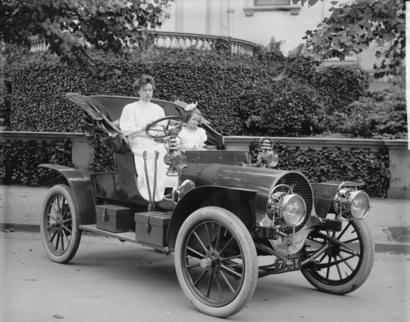
\includegraphics[width=\linewidth]{inc/sample-franklin}
%   \caption{1907 Franklin Model D roadster. Photograph by Harris \&
%     Ewing, Inc. [Public domain], via Wikimedia
%     Commons. (\url{https://goo.gl/VLCRBB}).}
%   \Description{A woman and a girl in white dresses sit in an open car.}
% \end{figure}

%% For a teaser figure.
% \begin{teaserfigure}
%   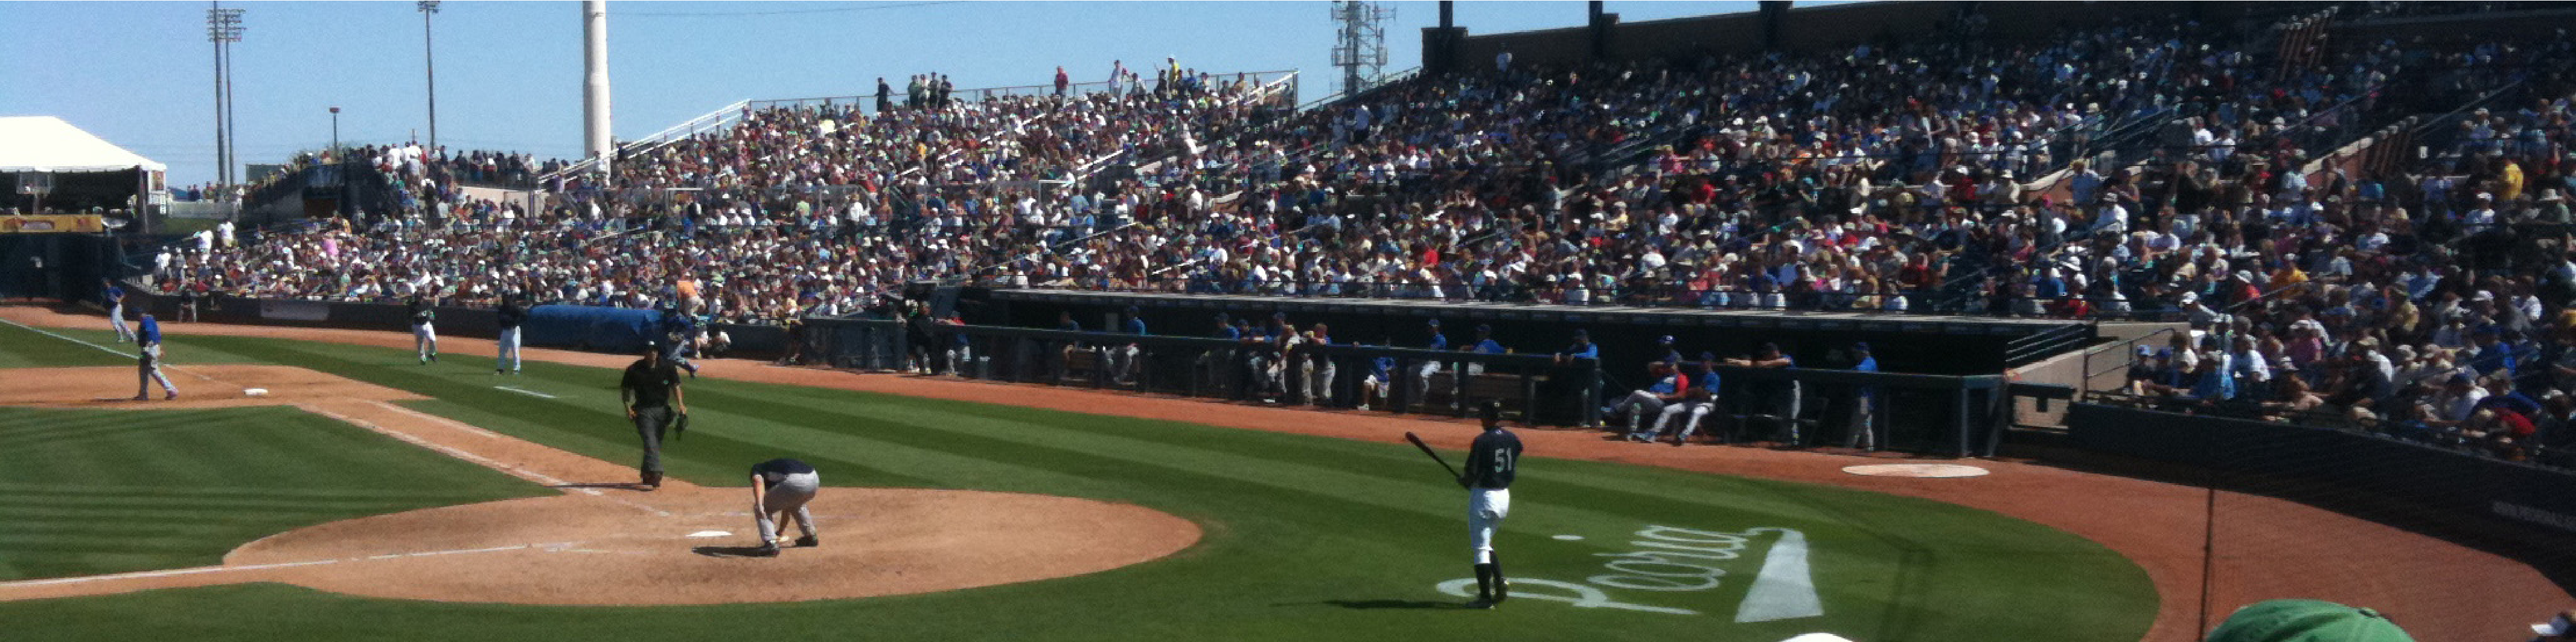
\includegraphics[width=\textwidth]{sampleteaser}
%   \caption{figure caption}
%   \Description{figure description}
% \end{teaserfigure}


\section{Related work}
\label{sec:related}
\ignore{Some of the early work on dynamic graph algorithms in the sequential setting include the seminal sparsification method of Eppstein et al. \cite{graph-eppstein97} and the bounded incremental computation idea of Ramalingam \cite{incr-ramalingam96}. The latter advocates measuring the work done as part of the update in proportion to the effect the update has on the computation.}

A number of approaches have been proposed for performing incremental computation (updating PageRank values in a dynamic / evolving graph) of approximate PageRank. Chien et al. \cite{rank-chien01} identify a tiny region of the graph near the updated vertices and model the remainder of the graph as a single vertex in a new, much smaller graph. PageRanks are computed for the small graph and then transferred to the original graph. Chen et al. \cite{chen2004local} propose a number of methods to estimate the PageRank score of a particular web page using only a small subgraph of the entire web, by expanding backwards from the target node following reverse hyperlinks. Bahmani et al. \cite{bahmani2010fast} analyze the efficiency of Monte Carlo methods for incremental computation of PageRank. Zhan et al. \cite{zhan2019fast} propose a Monte Carlo based algorithm for PageRank tracking on dynamic networks, by maintaining $R$ random walks starting from each node. Pashikanti et al. \cite{rank-pashikanti22} also follow a similar approach for updating PageRank scores on vertex and edge insertion/deletion.

A few approaches have been proposed for updating exact PageRank scores on dynamic graphs. Zhang \cite{rank-zhang17} presents a simple incremental Pagerank computation system for dynamic graphs on hybrid CPU and GPU platforms that incorporates the Update-Gather-Apply-Scatter (UGAS) computation model. A common approach used for Dynamic PageRank algorithm, given a small change to the input graph, is to find the affected region in the preprocessing step with Breadth-First Search (BFS) or Depth-First Search (DFS) traversal from the vertices connecting the edges that were inserted or deleted, and computing PageRanks only for that region \cite{rank-desikan05, kim2015incremental, rank-giri20, sahu2022dynamic}. This approach was originally proposed by Desikan et al. \cite{rank-desikan05}. Kim and Choi \cite{kim2015incremental} use this approach with an asynchronous implementation of PageRank. Giri et al. \cite{rank-giri20} use this approach with collaborative executions on muti-core CPUs and massively parallel GPUs. Sahu et al. \cite{sahu2022dynamic} use this approach on a Strongly Connected Component (SCC) based decomposition of the graph to limit the computation to SCCs that are reachable from updated vertices, on multi-core CPUs and GPUs (separately). Ohsaka et al. \cite{ohsaka2015efficient} propose an approach for locally updating PageRank using the Gauss-Southwell method, where the vertex with the greatest residual is updated first --- however, their algorithm is inherently sequential. 
%% Ohsaka et al. use L1-norm like many others for error.

% \ignore{PageRank algorithm is a \textbf{live algorithm} which means that an ongoing computation can be paused during graph update, and simply be resumed afterwards (instead of restarting it).} Dynamic PageRank algorithms aim to handle changes in the input graph efficiently.\ignore{A number of techniques have been proposed for online analysis of link evolution, i.e., updating of PageRank values in a dynamic/evolving graph.}

Further, Bahmani et al. \cite{rank-bahmani12} propose an algorithm to selectively crawl a small portion of the web to provide an estimate of true PageRank of the graph at that moment, while Berberich et al. \cite{rank-berberich07} present a method to compute normalized PageRank scores that are robust to non-local changes in the graph. Their approaches are orthogonal to our \textit{Dynamic Frontier} approach which focuses on the computation of the PageRank vector itself, not on the process of crawling the web or maintaining normalized scores.
%% Add other interesting variations?

%% We use an asynchronous approach:
% Real-Time PageRank on Dynamic Graphs (2023): In this paper, Sallinen et al. \cite{sallinen2023real} compute PageRank asynchronously for real-time, on demand PageRank computation with arbitrary granularity. They model PageRank as a flow problem, where mass is absorbed by the page, and the rest is distributed to neighbors. This is done by sending delta values of probability mass depending on edge deletion or insertions by adjustment upon earlier values. Sink/dangling vertices (dead ends) are handled as usual (teleport).

%% Interesting approach:
% PageRank Algorithm Based on Dynamic Damping Factor (2023): Existing methods often set the damping factor empirically, overlooking the relevance of web visitors’ topics. HaoLin et al. \cite{haolin2023pagerank} propose an adaptive dynamic damping factor based on the web browsing context, and demonstrate that it effectively mitigates the impact of noisy web pages on query results and improves the convergence speed.

%% Sliding window approach.
% Time-Aware Ranking in Dynamic Citation Networks (2011): In this paper, Ghosh et al. \cite{ghosh2011time} consider the temporal order of links and chains of links connecting to a node with some temporal decay factors, and show that it is more appropriate for predicting future citations and PageRank scores with regard to new citations.

%% Other interesting approach:
% A Dynamical System for PageRank with Time-Dependent Teleportation (2014): In this paper, Gleich and Rossi \cite{gleich2014dynamical} propose a time-dependent teleportation to the PageRank score. The magnitude of the deviation from a static PageRank vector is given by a PageRank problem with complex-valued teleportation parameters. They demonstrate the utility of dynamic teleportation on both the article graph of Wikipedia, where the external interest information is given by the number of hourly visitors to each page, and the Twitter social network, where external interest is the number of tweets per month. They show that using information from the dynamical system helps improve a prediction task and identify trends in the data.

%% Other interesting approach:
% Temporal PageRank (2016): In this paper, Rozenshtein and Gionis \cite{rozenshtein2016temporal} propose an extension of static PageRank to temporal PageRank so that only temporal walks are considered instead of all possible walks. In order to compute temporal PageRank we need to process the sequence of interactions and calculate the weighted number of temporal walks. Their algorithm counts explicitly the weighted number of temporal walks.

%% Similar to STIC-D:
% Divide and conquer approach for efficient pagerank computation (2006): In this paper, Desikan et al. \cite{desikan2006divide} propose a graph-partitioning technique for PageRank, on which computation can be performed independently.

%% Similar to STIC-D:
% A componentwise PageRank algorithm (2015): In this paper, Engstrom et al. \cite{engstrom2015componentwise} propose two PageRank algorithms, one similar to the Lumping algorithm proposed by Qing et al. which handles certain types of vertices faster, and last, another PageRank algorithm which can handle more types of vertices as well as strongly connected components more effectively. This is similar to the work of Garg et al.

%% Streaming PageRank:
% Estimating PageRank on graph streams (2011): In this paper, Sarma et al. \cite{rank-sarma11} study the streaming model for PageRank, which uses a small amount of memory (preferably sub-linear in the number of nodes n). They compute approximate PageRank values in Õ(nM−1/4) space and Õ(M3/4) passes. They also give another approach to approximate the PageRank values in just Õ(1) passes although this requires Õ(nM) space.

%% Applications of PageRank:
% PageRank Tracker: From Ranking to Tracking (2013): PageRank has been used by Gong et al. \cite{gong2013pagerank} in video object tracking to improve its robustness, i.e., to address difficulties with adaptation to environmental or target change. Determining the target is equivalent to finding the unlabeled sample that is the most associated with the existing labeled set.

%% Applications of PageRank:
% Abstracting PageRank To Dynamic Asset Valuation (2006): In this paper, Sawilla \cite{sawilla2006abstracting} uses (weighted) PageRank to quickly and dynamically calculate a relative value for all assets in an organization in any context in which dependencies may be specified. Their scheme works in general and will provide asset valuation in any context, be it confidentiality, integrity, availability, or even political capital.

%% For introduction, also a bit here:
% Adaptive Implementation to Update Page Rank on Dynamic Networks (2021): In this oral presentation, Srinivasan \cite{srinivasan2021adaptive} talk about the fact that There are a lot of attempts made to parallelize the page rank algorithm for static networks, however, there are only very few attempts made to compute page rank on dynamic networks. As the networks change with time, computing page rank or updating is an expensive operation, the previous attempts have only approximated the metric to avoid recomputation. In this paper, we introduce a framework where we try to update the page rank of the vertices which embraces change as the network changes. The proposed framework is implemented on a shared memory system and experiments on real-world and synthetic networks show good scalability. The framework proposed gets an input set of networks, initial page rank values for all the vertices, and a set of batches that has the changeset. As the batches are processed in parallel, affected vertices are identified and marked for an update, once the batch is processed the vertices affected or identified their page rank values are computed. The main contribution of this paper is the proposed framework avoids recomputation of all vertices, and only recomputes few vertices, and avoids approximation to provide accurate values.


\section{Preliminaries}
\label{sec:preliminaries}
Consider an undirected graph $G(V, E, w)$, where $V$ represents the set of vertices, $E$ the set of edges, and $w_{ij} = w_{ji}$ denotes the weight associated with each edge. In the case of an unweighted graph, we assume unit weight for each edge ($w_{ij} = 1$). Additionally, the neighbors of a vertex $i$ are denoted as $J_i = \{j\ |\ (i, j) \in E\}$, the weighted degree of each vertex as $K_i = \sum_{j \in J_i} w_{ij}$, the total number of vertices as $N = |V|$, the total number of edges as $M = |E|$, and the sum of edge weights in the undirected graph as $m = \sum_{i, j \in V} w_{ij}/2$.




\subsection{Community detection}

Disjoint community detection involves identifying a community membership mapping, $C: V \rightarrow \Gamma$, where each vertex $i \in V$ is assigned a community-id $c$ from the set of community-ids $\Gamma$. We denote the vertices of a community $c \in \Gamma$ as $V_c$, and the community that a vertex $i$ belongs to as $C_i$. Further, we denote the neighbors of vertex $i$ belonging to a community $c$ as $J_{i \rightarrow c} = \{j\ |\ j \in J_i\ and\ C_j = c\}$, the sum of those edge weights as $K_{i \rightarrow c} = \sum_{j \in J_{i \rightarrow c}} w_{ij}$, the sum of weights of edges within a community $c$ as $\sigma_c = \sum_{(i, j) \in E\ and\ C_i = C_j = c} w_{ij}$, and the total edge weight of a community $c$ as $\Sigma_c = \sum_{(i, j) \in E\ and\ C_i = c} w_{ij}$ \cite{com-leskovec21}.




\subsection{Modularity}

Modularity serves as a\ignore{fitness} metric for evaluating the quality of communities identified by heuristic-based community detection algorithms. It is calculated as the difference between the fraction of edges within communities and the expected fraction if edges were randomly distributed, yielding a range of $[-0.5, 1]$, where higher values signify superior results \cite{com-brandes07}.\ignore{The optimization of this metric theoretically leads to the optimal grouping \cite{com-newman04, com-traag11}.} The modularity $Q$ of identified communities is determined using Equation \ref{eq:modularity}, where $\delta$ represents the Kronecker delta function ($\delta (x,y)=1$ if $x=y$, $0$ otherwise). The \textit{delta modularity} of moving a vertex $i$ from community $d$ to community $c$, denoted as $\Delta Q_{i: d \rightarrow c}$, can be calculated using Equation \ref{eq:delta-modularity}.

\begin{equation}
\label{eq:modularity}
  Q
  = \frac{1}{2m} \sum_{(i, j) \in E} \left[w_{ij} - \frac{K_i K_j}{2m}\right] \delta(C_i, C_j)
  = \sum_{c \in \Gamma} \left[\frac{\sigma_c}{2m} - \left(\frac{\Sigma_c}{2m}\right)^2\right]
\end{equation}

\begin{equation}
\label{eq:delta-modularity}
  \Delta Q_{i: d \rightarrow c}
  = \frac{1}{m} (K_{i \rightarrow c} - K_{i \rightarrow d}) - \frac{K_i}{2m^2} (K_i + \Sigma_c - \Sigma_d)
\end{equation}




\subsection{Louvain algorithm}
\label{sec:about-louvain}

The Louvain method \cite{com-blondel08} is an agglomerative algorithm that optimizes modularity to identify high quality disjoint communities in large networks. It has a time complexity of $O (L |E|)$, where $L$ is the total number of iterations performed, and a space complexity of $O(|V| + |E|)$ \cite{com-lancichinetti09}. This algorithm comprises two phases: the \textit{local-moving phase}, in which each vertex $i$ greedily decides to join the community of one of its neighbors $j \in J_i$ to maximize the increase in modularity $\Delta Q_{i:C_i \rightarrow C_j}$ (using Equation \ref{eq:delta-modularity}), and the \textit{aggregation phase}, where all vertices in a community are merged into a single super-vertex. These phases constitute one pass, which is repeated until there is no further increase in modularity is observed \cite{com-blondel08, com-leskovec21}.\ignore{We observe that Louvain obtains high-quality communities, with $3.0 - 30\%$ higher modularity than that obtained by LPA, but requires $2.3 - 14\times$ longer to converge.}




\subsection{Leiden algorithm}
\label{sec:about-leiden}

As mentioned earlier, the Louvain method, while effective, may identify internally disconnected communities and arbitrarily badly connected ones. Traag et al. \cite{com-traag19} proposed the Leiden algorithm to address these issues. The algorithm introduces a \textit{refinement phase} subsequent to the local-moving phase, wherein vertices within each community undergo additional updates to their community membership within their community bounds (obtained from the local-moving phase), starting from a singleton community. This is performed in a randomized manner, with the probability of joining a neighboring community within its community bound being proportional to the delta-modularity of the move. This facilitates the identification of sub-communities within those obtained from the local-moving phase. The Leiden algorithm not only guarantees that all communities are well separated (akin to the Louvain method), but also are well connected. Once communities have converged, it is guaranteed that all vertices are optimally assigned, and all communities are subset optimal \cite{com-traag19}. It has a time complexity of $O (L |E|)$, where $L$ is the total number of iterations performed, and a space complexity of $O(|V| + |E|)$, similar to the Louvain method.


\section{Approach}
\label{sec:approach}
\subsection{Optimizations for Leiden algorithm}
\label{sec:leiden}

We extend our optimization techniques, originally designed for the Louvain method \cite{sahu2023gvelouvain}, to the Leiden algorithm. Specifically, we implement an \textit{asynchronous} version of the Leiden algorithm, allowing threads to operate independently on distinct sections of the graph. While this approach promotes faster convergence, it also introduces variability into the final result \cite{com-shi21}. To ensure efficient computations, we allocate a dedicated hashtable per thread. These hashtables serve two main purposes: they keep track of the delta-modularity associated with moving to each community connected to a vertex during the local-moving/refinement phases, and they record the total edge weight between super-vertices in the aggregation phase of the algorithm \cite{sahu2023gvelouvain}.

Our optimizations encompass several strategies, including utilizing OpenMP's \textit{dynamic} loop scheduling, capping the number of iterations per pass at $20$, employing a tolerance drop rate of $10$ (threshold scaling), initiating with a tolerance of $0.01$, using an aggregation tolerance of $0.8$ to avoid performing aggregations of minimal utility, implementing flag-based vertex pruning (instead of a queue-based one \cite{nguyenleiden}), utilizing parallel prefix sum, and using preallocated Compressed Sparse Row (CSR) data structures for identifying community vertices and storing the super-vertex graph during aggregation. Additionally, we employ fast collision-free per-thread hashtables, well separated in their memory addresses \cite{sahu2023gvelouvain}.

We attempt two approaches of the Leiden algorithm. One uses a \textit{greedy refinement phase} where vertices greedily optimize for delta-modularity (within their community bounds), while the other uses a \textit{randomized refinement phase} (using fast \textit{xorshift32} random number generators), where the likelihood of selection of a community to move to (by a vertex) is proportional to its delta-modularity, as originally proposed \cite{com-traag19}. Our results, shown in Figures \ref{fig:leidenopt-runtime} and \ref{fig:leidenopt-modularity}, indicate the \textit{greedy approach} performs the best on average, both in terms of runtime and modularity. We also try medium and heavy variants for both approaches, which disables threshold scaling and aggregation tolerance (including threshold scaling) respectively, However, we do not find them to perform well overall.\ignore{On \textit{europe\_osm} graph, our parallel Greedy-Leiden (which we from here on refer to simply as Leiden) runs $3\times$ faster than Nguyen \cite{nguyenleiden}.}

\ignore{We fixed a bug that caused the Leiden algorithm to fail in finding communities on road networks and kmer graphs. The issue was forgetting to reset the affected vertices flags before running the refinement phase.}

\begin{figure}[hbtp]
  \centering
  \subfigure{
    \label{fig:leidenopt-runtime--all}
    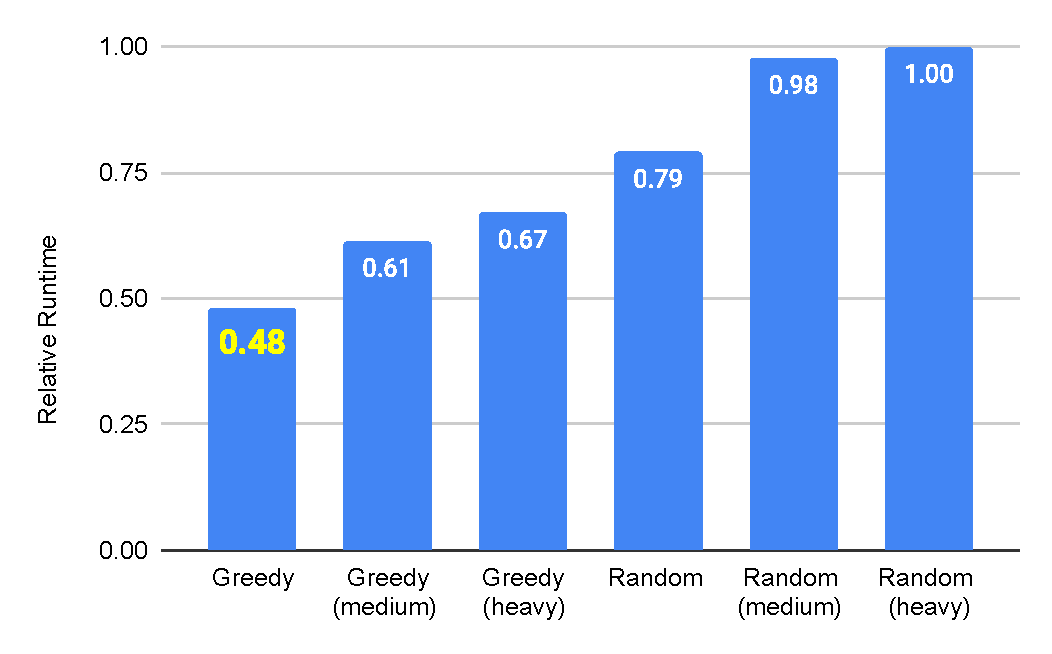
\includegraphics[width=0.98\linewidth]{out/leidenopt-runtime.pdf}
  } \\[-2ex]
  \caption{Average relative runtime for the \textit{greedy} and \textit{random} approaches (including \textit{medium} and \textit{heavy} variants) of parallel Leiden algorithm for all graphs in the dataset.}
  \label{fig:leidenopt-runtime}
\end{figure}

\begin{figure}[hbtp]
  \centering
  \subfigure{
    \label{fig:leidenopt-modularity--all}
    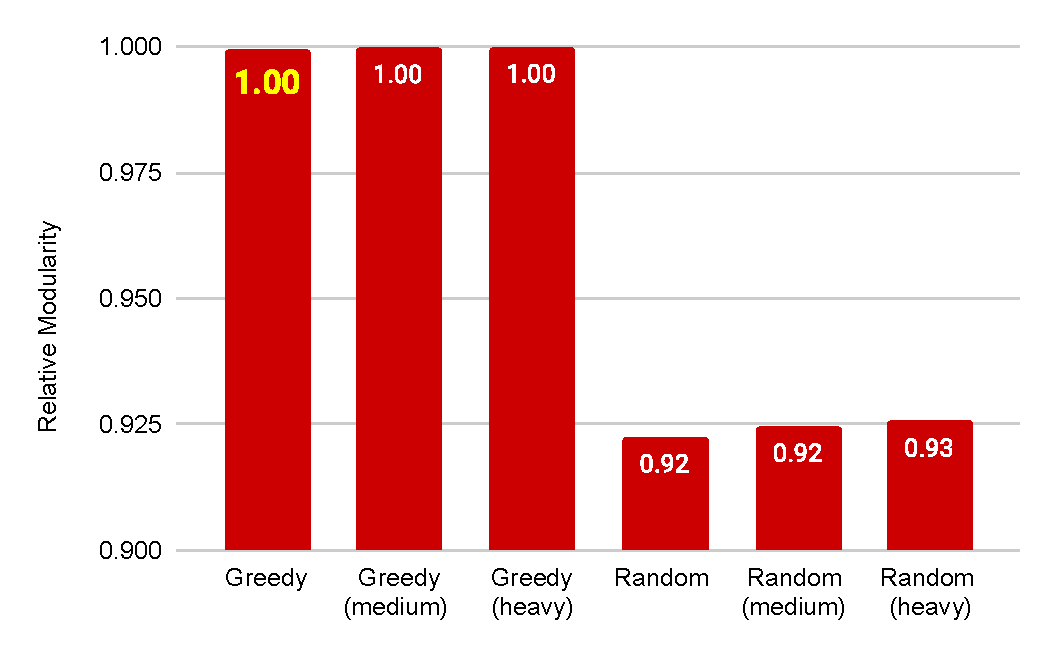
\includegraphics[width=0.98\linewidth]{out/leidenopt-modularity.pdf}
  } \\[-2ex]
  \caption{Average relative modularity for the \textit{greedy} and \textit{random} approaches (including \textit{medium} and \textit{heavy} variants) of parallel Leiden algorithm for all graphs in the dataset.}
  \label{fig:leidenopt-modularity}
\end{figure}

\begin{figure*}[hbtp]
  \centering
  \subfigure{
    \label{fig:leiden-pass--all}
    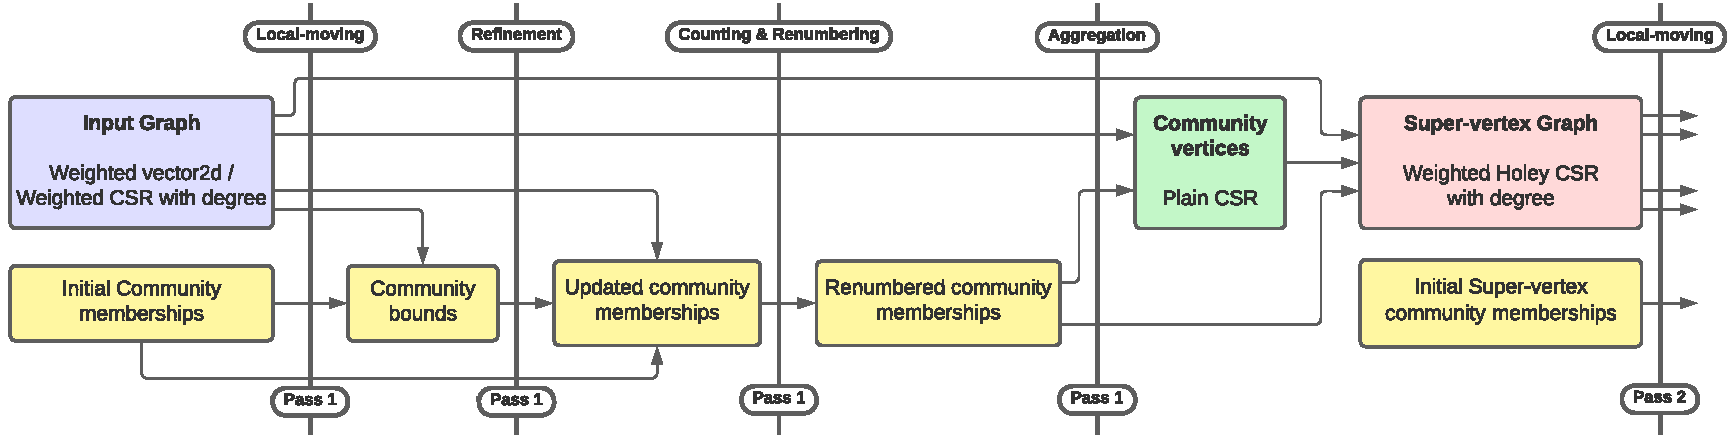
\includegraphics[width=0.98\linewidth]{out/leiden-pass.pdf}
  } \\[-2ex]
  \caption{A flow diagram illustrating the first pass of GVE-Leiden for either a Weighted 2D-vector-based or a Weighted CSR with degree-based input graph. In the local-moving phase, vertex community memberships are updated to obtain community bounds for the refinement phase, until the cumulative delta-modularity change across all vertices reaches a specified threshold. Then, in the refinement phase, the each vertex starts in a singleton community, and community memberships are updated similarly to the local-moving phase, with vertices changing communities within their bounds. These community memberships are then counted and renumbered. In the aggregation phase, community vertices in a CSR are first obtained. This is used to create the super-vertex graph stored in a Weighted Holey CSR with degree. Subsequent passes use a Weighted Holey CSR with degree and initial community memberships for super-vertices from the previous pass as input.}
  \label{fig:leiden-pass}
\end{figure*}





\subsection{Our optimized Leiden implementation}

We now explain the implementation of GVE-Leiden in Algorithms \ref{alg:leiden}, \ref{alg:leidenlm}, \ref{alg:leidenre}, and \ref{alg:leidenag}. A flow diagram illustrating the first pass of GVE-Leiden is shown in Figure \ref{fig:leiden-pass}.


\subsubsection{Main step of GVE-Leiden}

The main step of GVE-Leiden (\texttt{leiden()} function) is outlined in Algorithm \ref{alg:leiden}. It encompasses initialization, the local-moving phase, the refinement phase, and the aggregation phase. Here, the \texttt{leiden()} function accepts the input graph $G$, and returns the community membership $C$ of each vertex. In line \ref{alg:leiden--initialization}, we first initialize the community membership $C$ for each vertex in $G$, and perform passes of the Leiden algorithm, limited to $MAX\_PASSES$ (lines \ref{alg:leiden--passes-begin}-\ref{alg:leiden--passes-end}). During each pass, we initialize the total edge weight of each vertex $K'$, the total edge weight of each community $\Sigma'$, and the community membership $C'$ of each vertex in the current graph $G'$ (line \ref{alg:leiden--reset-weights}).

Subsequently, in line \ref{alg:leiden--local-move}, we perform the local-moving phase by invoking \texttt{leidenMove()} (Algorithm \ref{alg:leidenlm}), which optimizes community assignments. Following this, we set the \textit{community bound} of each vertex (for the refinement phase) as the community membership of each vertex just obtained, and reset the membership of each vertex, and the total weight of each community as singleton vertices in line \ref{alg:leiden--reset-again}. In line \ref{alg:leiden--refine}, the refinement phase is carried out by invoking \texttt{leidenRefine()} (Algorithm \ref{alg:leidenre}), which optimizes the community assignment of each vertex within its community bound. If either the local-moving or the refinement phase converged in a single iteration, global convergence is implied and we terminate the passes (line \ref{alg:leiden--globally-converged}). Further, if the drop in community count $|\Gamma|$ is marginal, we halt at the current pass (line \ref{alg:leiden--aggregation-tolerance}).

If convergence has not been achieved, we proceed to renumber communities (line \ref{alg:leiden--renumber}), update top-level community memberships $C$ with dendrogram lookup (line \ref{alg:leiden--lookup}), perform the aggregation phase by calling \texttt{leidenAggregate()} (Algorithm \ref{alg:leidenag}), and adjust the convergence threshold for subsequent passes, i.e., perform threshold scaling (line \ref{alg:leiden--threshold-scaling}). The next pass commences in line \ref{alg:leiden--passes-begin}. At the end of all passes, we perform a final update of the top-level community memberships $C$ with dendrogram lookup (line \ref{alg:leiden--lookup-last}), and return the top-level community membership $C$ of each vertex in $G$.

\begin{algorithm}[hbtp]
\caption{GVE-Leiden: Our parallel Leiden algorithm.}
\label{alg:leiden}
\begin{algorithmic}[1]
\Require{$G$: Input graph}
\Require{$C$: Community membership of each vertex}
\Require{$G'$: Input/super-vertex graph}
\Require{$C'$: Community membership of each vertex in $G'$}
\Require{$K'$: Total edge weight of each vertex}
\Require{$\Sigma'$: Total edge weight of each community}
\Ensure{$G'_{C'}$: Community vertices (CSR)}
\Ensure{$H_t$: Collision-free per-thread hashtable}
\Ensure{$l_i$, $l_j$: Number of iterations performed (per pass)}
\Ensure{$l_p$: Number of passes performed}
\Ensure{$\tau$: Per iteration tolerance}
\Ensure{$\tau_{agg}$: Aggregation tolerance}

\Statex

\Function{leiden}{$G$} \label{alg:leiden--begin}
  \State Vertex membership: $C \gets [0 .. |V|)$ \textbf{;} $G' \gets G$ \label{alg:leiden--initialization}
  \ForAll{$l_p \in [0 .. \text{\small{MAX\_PASSES}})$} \label{alg:leiden--passes-begin}
    \State $\Sigma' \gets K' \gets vertexWeights(G')$ \textbf{;} $C' \gets [0 .. |V'|)$ \label{alg:leiden--reset-weights}
    \State $l_i \gets leidenMove(G', C', K', \Sigma', \tau)$ \label{alg:leiden--local-move}
    \State $C'_B \gets C'$ \textbf{;} $C' \gets [0 .. |V'|)$ \textbf{;} $\Sigma' \gets K'$ \label{alg:leiden--reset-again}
    \State $l_j \gets leidenRefine(G', C'_B, C', K', \Sigma', \tau)$ \label{alg:leiden--refine}
    \If{$l_i + l_j \le 1$} \textbf{break} \Comment{Globally converged?} \label{alg:leiden--globally-converged}
    \EndIf
    \State $|\Gamma|, |\Gamma_{old}| \gets$ Number of communities in $C$, $C'$
    \If{$|\Gamma|/|\Gamma_{old}| > \tau_{agg}$} \textbf{break} \Comment{Low shrink?} \label{alg:leiden--aggregation-tolerance}
    \EndIf
    \State $C' \gets$ Renumber communities in $C'$ \label{alg:leiden--renumber}
    \State $C \gets$ Lookup dendrogram using $C$ to $C'$ \label{alg:leiden--lookup}
    \State $G' \gets leidenAggregate(G', C')$ \label{alg:leiden--aggregate}
    \State $\tau \gets \tau / \text{\small{TOLERANCE\_DROP}}$ \Comment{Threshold scaling} \label{alg:leiden--threshold-scaling}
  \EndFor \label{alg:leiden--passes-end}
  \State $C \gets$ Lookup dendrogram using $C$ to $C'$ \label{alg:leiden--lookup-last}
  \Return{$C$} \label{alg:leiden--return}
\EndFunction \label{alg:leiden--end}
\end{algorithmic}
\end{algorithm}

\begin{algorithm}[hbtp]
\caption{Local-moving phase of GVE-Leiden.}
\label{alg:leidenlm}
\begin{algorithmic}[1]
\Require{$G'$: Input/super-vertex graph}
\Require{$C'$: Community membership of each vertex}
\Require{$K'$: Total edge weight of each vertex}
\Require{$\Sigma'$: Total edge weight of each community}
\Ensure{$G'_{C'}$: Community vertices (CSR)}
\Ensure{$H_t$: Collision-free per-thread hashtable}
\Ensure{$l_i$: Number of iterations performed}
\Ensure{$\tau$: Per iteration tolerance}

\Statex

\Function{leidenMove}{$G', C', K', \Sigma', \tau$} \label{alg:leidenlm--move-begin}
  \State Mark all vertices in $G'$ as unprocessed \label{alg:leidenlm--reset-affected}
  \ForAll{$l_i \in [0 .. \text{\small{MAX\_ITERATIONS}})$} \label{alg:leidenlm--iterations-begin}
    \State Total delta-modularity per iteration: $\Delta Q \gets 0$ \label{alg:leidenlm--init-deltaq}
    \ForAll{unprocessed $i \in V'$ \textbf{in parallel}} \label{alg:leidenlm--loop-vertices-begin}
      \State Mark $i$ as processed (prune) \label{alg:leidenlm--prune}
      \State $H_t \gets scanCommunities(\{\}, G', C', i, false)$ \label{alg:leidenlm--scan}
      \State $\rhd$ Use $H_t, K', \Sigma'$ to choose best community
      \State $c^* \gets$ Best community linked to $i$ in $G'$ \label{alg:leidenlm--best-community-begin}
      \State $\delta Q^* \gets$ Delta-modularity of moving $i$ to $c^*$ \label{alg:leidenlm--best-community-end}
      \If{$c^* = C'[i]$} \textbf{continue} \label{alg:leidenlm--best-community-same}
      \EndIf
      \State $\Sigma'[C'[i]] -= K'[i]$ \textbf{;} $\Sigma'[c^*] += K'[i]$ \textbf{atomic} \label{alg:leidenlm--perform-move-begin}
      \State $C'[i] \gets c^*$ \textbf{;} $\Delta Q \gets \Delta Q + \delta Q^*$ \label{alg:leidenlm--perform-move-end}
      \State Mark neighbors of $i$ as unprocessed \label{alg:leidenlm--remark}
    \EndFor \label{alg:leidenlm--loop-vertices-end}
    \If{$\Delta Q \le \tau$} \textbf{break} \Comment{Locally converged?} \label{alg:leidenlm--locally-converged}
    \EndIf
  \EndFor \label{alg:leidenlm--iterations-end}
  \Return{$l_i$} \label{alg:leidenlm--return}
\EndFunction \label{alg:leidenlm--move-end}

\Statex

\Function{scanCommunities}{$H_t, G', C', i, self$}
  \ForAll{$(j, w) \in G'.edges(i)$}
    \If{\textbf{not} $self$ \textbf{and} $i = j$} \textbf{continue}
    \EndIf
    \State $H_t[C'[j]] \gets H_t[C'[j]] + w$
  \EndFor
  \Return{$H_t$}
\EndFunction
\end{algorithmic}
\end{algorithm}

\begin{algorithm}[hbtp]
\caption{Refinement phase of GVE-Leiden.}
\label{alg:leidenre}
\begin{algorithmic}[1]
\Require{$G'$: Input/super-vertex graph}
\Require{$C'$: Community membership of each vertex}
\Require{$K'$: Total edge weight of each vertex}
\Require{$\Sigma'$: Total edge weight of each community}
\Ensure{$G'_{C'}$: Community vertices (CSR)}
\Ensure{$H_t$: Collision-free per-thread hashtable}
\Ensure{$l_j$: Number of iterations performed}
\Ensure{$\tau$: Per iteration tolerance}

\Statex

\Function{leidenRefine}{$G', C'_B, C', K', \Sigma', \tau$} \label{alg:leidenre--move-begin}
  \State Mark all vertices in $G'$ as unprocessed \label{alg:leidenre--reset-affected}
  \ForAll{$l_j \in [0 .. \text{\small{MAX\_ITERATIONS}})$} \label{alg:leidenre--iterations-begin}
    \State Total delta-modularity per iteration: $\Delta Q \gets 0$ \label{alg:leidenre--init-deltaq}
    \ForAll{unprocessed $i \in V'$ \textbf{in parallel}} \label{alg:leidenre--loop-vertices-begin}
      \State Mark $i$ as processed (prune) \label{alg:leidenre--prune}
      \State $H_t \gets scanBounded(\{\}, G', C'_B, C', i, false)$ \label{alg:leidenre--scan}
      \State $\rhd$ Use $H_t, K', \Sigma'$ to choose best community
      \State $c^* \gets$ Best community linked to $i$ in $G'$ within $C'_B$ \label{alg:leidenre--best-community-begin}
      \State $\delta Q^* \gets$ Delta-modularity of moving $i$ to $c^*$ \label{alg:leidenre--best-community-end}
      \If{$c^* = C'[i]$} \textbf{continue} \label{alg:leidenre--best-community-same}
      \EndIf
      \State $\Sigma'[C'[i]] -= K'[i]$ \textbf{;} $\Sigma'[c^*] += K'[i]$ \textbf{atomic} \label{alg:leidenre--perform-move-begin}
      \State $C'[i] \gets c^*$ \textbf{;} $\Delta Q \gets \Delta Q + \delta Q^*$ \label{alg:leidenre--perform-move-end}
      \State Mark neighbors of $i$ as unprocessed \label{alg:leidenre--remark}
    \EndFor \label{alg:leidenre--loop-vertices-end}
    \If{$\Delta Q \le \tau$} \textbf{break} \Comment{Locally converged?} \label{alg:leidenre--locally-converged}
    \EndIf
  \EndFor \label{alg:leidenre--iterations-end}
  \Return{$l_j$} \label{alg:leidenre--return}
\EndFunction \label{alg:leidenre--move-end}

\Statex

\Function{scanBounded}{$H_t, G', C'_B, C', i, self$}
  \ForAll{$(j, w) \in G'.edges(i)$}
    \If{\textbf{not} $self$ \textbf{and} $i = j$} \textbf{continue}
    \EndIf
    \If{$C'_B[i] \neq C'_B[j]$} \textbf{continue}
    \EndIf
    \State $H_t[C'[j]] \gets H_t[C'[j]] + w$
  \EndFor
  \Return{$H_t$}
\EndFunction
\end{algorithmic}
\end{algorithm}

\begin{algorithm}[hbtp]
\caption{Aggregation phase of GVE-Leiden.}
\label{alg:leidenag}
\begin{algorithmic}[1]
\Require{$G'$: Input/super-vertex graph}
\Require{$C'$: Community membership of each vertex}
\Ensure{$G'_{C'}$: Community vertices (CSR)}
\Ensure{$G''$: Super-vertex graph (weighted CSR)}
\Ensure{$*.offsets$: Offsets array of a CSR graph}
\Ensure{$H_t$: Collision-free per-thread hashtable}

\Statex

\Function{leidenAggregate}{$G', C'$}
  \State $\rhd$ Obtain vertices belonging to each community
  \State $G'_{C'}.offsets \gets countCommunityVertices(G', C')$ \label{alg:leidenag--coff-begin}
  \State $G'_{C'}.offsets \gets exclusiveScan(G'_{C'}.offsets)$ \label{alg:leidenag--coff-end}
  \ForAll{$i \in V'$ \textbf{in parallel}} \label{alg:leidenag--comv-begin}
    \State Add edge $(C'[i], i)$ to CSR $G'_{C'}$ atomically
  \EndFor \label{alg:leidenag--comv-end}
  \State $\rhd$ Obtain super-vertex graph
  \State $G''.offsets \gets communityTotalDegree(G', C')$ \label{alg:leidenag--yoff-begin}
  \State $G''.offsets \gets exclusiveScan(G''.offsets)$ \label{alg:leidenag--yoff-end}
  \State $|\Gamma| \gets$ Number of communities in $C'$
  \ForAll{$c \in [0, |\Gamma|)$ \textbf{in parallel}} \label{alg:leidenag--y-begin}
    \If{degree of $c$ in $G'_{C'} = 0$} \textbf{continue}
    \EndIf
    \State $H_t \gets \{\}$
    \ForAll{$i \in G'_{C'}.edges(c)$}
      \State $H_t \gets scanCommunities(H, G', C', i, true)$
    \EndFor
    \ForAll{$(d, w) \in H_t$}
      \State Add edge $(c, d, w)$ to CSR $G''$ atomically
    \EndFor
  \EndFor \label{alg:leidenag--y-end}
  \Return $G''$ \label{alg:leidenag--return}
\EndFunction
\end{algorithmic}
\end{algorithm}



\subsubsection{Local-moving phase of GVE-Leiden}

The pseuodocode for the local-moving phase of GVE-Leiden is shown in Algorithm \ref{alg:leidenlm}, which iteratively moves vertices between communities to maximize modularity. Here, the \texttt{leidenMove()} function takes the current graph $G'$, community membership $C'$, total edge weight of each vertex $K'$ and each community $\Sigma'$, the iteration tolerance $\tau$ as input, and returns the number of iterations performed $l_i$.

Lines \ref{alg:leidenlm--iterations-begin}-\ref{alg:leidenlm--iterations-end} represent the main loop of the local-moving phase. In line \ref{alg:leidenlm--reset-affected}, we first mark all vertices as unprocessed. Then, in line \ref{alg:leidenlm--init-deltaq}, we initialize the total delta-modularity per iteration $\Delta Q$. Next, in lines \ref{alg:leidenlm--loop-vertices-begin}-\ref{alg:leidenlm--loop-vertices-end}, we iterate over unprocessed vertices in parallel. For each unprocessed vertex $i$, we mark $i$ as processed - vertex pruning (line \ref{alg:leidenlm--prune}), scan communities connected to $i$ - excluding self (line \ref{alg:leidenlm--scan}), determine the best community $c*$ to move $i$ to (line \ref{alg:leidenlm--best-community-begin}), and calculate the delta-modularity of moving $i$ to $c*$ (line \ref{alg:leidenlm--best-community-end}). We then update the community membership of $i$ (lines \ref{alg:leidenlm--perform-move-begin}-\ref{alg:leidenlm--perform-move-end}) and mark its neighbors as unprocessed (line \ref{alg:leidenlm--remark}) if a better community was found. In line \ref{alg:leidenlm--locally-converged}, we check if the local-moving phase has converged. If so, we break out of the loop (or if $MAX\_ITERATIONS$ is reached). At the end, in line \ref{alg:leidenlm--return}, we return the number of iterations performed $l_i$.


\subsubsection{Refinement phase of GVE-Leiden}

The pseuodocode for the refinement phase of GVE-Leiden is presented in Algorithm \ref{alg:leidenlm}. This is similar to the local-moving phase, but utilizes the obtained community membership of each vertex as a \textit{community bound}, where each vertex must choose to join the community of another vertex within its community bound.\ignore{Similar to the local-moving phase however, vertices iteratively move between communities to maximize modularity.} At the start of the refinement phase, the community membership of each vertex is reset, such that each vertex belongs to its own community. Here, the \texttt{leidenRefine()} function takes the current graph $G'$, the community bound of each vertex $C'_B$, the initial community membership $C'$ of each vertex, the total edge weight of each vertex $K'$, the initial total edge weight of each community $\Sigma'$, and the current per iteration tolerance $\tau$ as input, and returns the number of iterations performed $l_j$.

Lines \ref{alg:leidenre--iterations-begin}-\ref{alg:leidenre--iterations-end} represent the core of the refinement phase. First, we initialize all vertices as unprocessed (line \ref{alg:leidenre--reset-affected}). Subsequently, we initialize the per-iteration delta-modularity $\Delta Q$ (line \ref{alg:leidenre--init-deltaq}), and iterate over unprocessed vertices in parallel (lines \ref{alg:leidenre--loop-vertices-begin}-\ref{alg:leidenre--loop-vertices-end}). For each unprocessed vertex $i$, we prune $i$ (line \ref{alg:leidenre--prune}), scan communities connected to $i$ within the \textit{same community bound} - excluding self (line \ref{alg:leidenre--scan}), evaluate the best community $c*$ to move $i$ to (line \ref{alg:leidenre--best-community-begin}), and compute the delta-modularity of moving $i$ to $c*$ (line \ref{alg:leidenre--best-community-end}). If a better community was found, we update the community membership (lines \ref{alg:leidenre--perform-move-begin}-\ref{alg:leidenre--perform-move-end}) of $i$, and mark its neighbors as unprocessed (line \ref{alg:leidenre--remark}). In line \ref{alg:leidenre--locally-converged}, we check if the refinement phase has converged. If so, we stop iterating (or if $MAX\_ITERATIONS$ is reached). Finally, we return the number of iterations performed $l_j$ (line \ref{alg:leidenre--return}).

\begin{algorithm}[hbtp]
\caption{Finding disconnected communities in parallel.}
\label{alg:disconnected}
\begin{algorithmic}[1]
\Require{$G$: Input graph}
\Require{$C$: Community membership of each vertex}
\Ensure{$D$: Disconnected flag for each community}
\Ensure{$S$: Size of each community}
\Ensure{$f_{if}$: Perform BFS to vertex $j$ if condition satisfied}
\Ensure{$f_{do}$: Perform operation after each vertex is visited}
\Ensure{$reached$: Number of vertices reachable from $i$ to $i$'s community}
\Ensure{$work_t$: Work-list of current thread}

\Statex

\Function{disconnectedCommunities}{$G, C$} \label{alg:disconnected--begin}
  \State $D \gets \{\}$ \textbf{;} $vis \gets \{\}$ \label{alg:disconnected--init}
  \State $S \gets communitySizes(G, C)$ \label{alg:disconnected--sizes}
  \ForAll{\textbf{threads in parallel}} \label{alg:disconnected--threads-begin}
    \ForAll{$i \in V$} \label{alg:disconnected--loop-begin}
      \State $c \gets C[i]$ \textbf{;} $reached \gets 0$ \label{alg:disconnected--unreached}
      \State $\rhd$ Skip if community $c$ is empty, or
      \State $\rhd$ does not belong to work-list of current thread.
      \If{$S[c] = 0$ \textbf{or} $c \notin work_t$} \textbf{continue} \label{alg:disconnected--work}
      \EndIf
      \State $f_{if} \gets (j) \implies C[j] = c$
      \State $f_{do} \gets (j) \implies reached \gets reached + 1$
      \State $bfsVisitForEach(vis, G, i, f_{if}, f_{do})$ \label{alg:disconnected--bfs}
      \If{$reached < S[c]$} $D[c] \gets 1$ \label{alg:disconnected--mark}
      \EndIf
      \State $S[c] \gets 0$ \label{alg:disconnected--processed}
    \EndFor \label{alg:disconnected--loop-end}
  \EndFor \label{alg:disconnected--threads-end}
  \Return{$D$}
\EndFunction \label{alg:disconnected--end}
\end{algorithmic}
\end{algorithm}



\subsubsection{Aggregation phase of GVE-Leiden}

Finally, we show the psuedocode for the aggregation phase in Algorithm \ref{alg:leidenag}, where communities are aggregated into super-vertices in preparation for the next pass of the Leiden algorithm (which operates on the super-vertex graph). Here, the \texttt{leidenAggregate()} function takes the current graph $G'$ and the community membership $C'$ as input, and returns the super-vertex graph $G''$.

In lines \ref{alg:leidenag--coff-begin}-\ref{alg:leidenag--coff-end}, the offsets array for the community vertices CSR $G'_{C'}.offsets$ is obtained. This is achieved by initially counting the number of vertices in each community using \texttt{countCommunityVert} \texttt{ices()} and subsequently performing an exclusive scan on the array. In lines \ref{alg:leidenag--comv-begin}-\ref{alg:leidenag--comv-end},  a parallel iteration over all vertices is performed to atomically populate vertices belonging to each community into the community graph CSR $G'_{C'}$. Following this, the offsets array for the super-vertex graph CSR is obtained by overestimating the degree of each super-vertex. This involves calculating the total degree of each community with \texttt{communityTotalDegree()} and performing an exclusive scan on the array (lines \ref{alg:leidenag--yoff-begin}-\ref{alg:leidenag--yoff-end}). As a result, the super-vertex graph CSR becomes holey, featuring gaps between the edges and weights arrays of each super-vertex in the CSR.

Then, in lines \ref{alg:leidenag--y-begin}-\ref{alg:leidenag--y-end}, a parallel iteration over all communities $c \in [0, |\Gamma|)$ is performed. For each vertex $i$ belonging to community $c$, all communities $d$ (with associated edge weight $w$), linked to $i$ as defined by \texttt{scanCommunities()} in Algorithm \ref{alg:leidenlm}, are added to the per-thread hashtable $H_t$. Once $H_t$ is populated with all communities (and associated weights) linked to community $c$, these are atomically added as edges to super-vertex $c$ in the super-vertex graph $G''$. Finally, in line \ref{alg:leidenag--return}, we return the super-vertex graph $G''$.




\subsection{Finding disconnected communities}

We now outline our parallel algorithm for identifying disconnected communities, given the original graph and the community membership of each vertex. The core concept involves determining the size of each community, selecting a vertex from each community, traversing within the community from that vertex (avoiding adjacent communities), and marking a community as disconnected if all its vertices cannot be reached. We explore four distinct approaches, differing in the use of parallel Depth-First Search (DFS) or Breadth-First Search (BFS) and whether per-thread or shared \textit{visited} flags are employed. If shared visited flags are used, each thread scans all vertices but processes only its assigned community based on the community ID. Our findings suggest that utilizing parallel BFS traversal with a shared flag vector yields the fastest results. As this is not a heuristic algorithm, all approaches produce identical outcomes. Algorithm \ref{alg:disconnected} illustrates the pseudocode for this approach. Here, the \texttt{disconnectedCommunities()} function takes the input graph $G$ and the community membership $C$ as input, and it returns the disconnected flag $D$ for each community.

We now explain Algorithm \ref{alg:disconnected} in detail. First, in line \ref{alg:disconnected--init}, the disconnected community flag $D$, and the visited vertices flags $vis$ are initialized. In line \ref{alg:disconnected--sizes}, the size of each community $S$ is obtained in parallel using the \texttt{communitySizes()} function. Subsequently, each thread processes each vertex $i$ in the graph $G$ in parallel (lines \ref{alg:disconnected--loop-begin}-\ref{alg:disconnected--loop-end}). In line \ref{alg:disconnected--unreached}, the community membership of $i$ ($c$) is determined, and the count of vertices reached from $i$ is initialized to $0$. If community $c$ is empty or not in the work-list of the current thread $work_t$, the thread proceeds to the next iteration (line \ref{alg:disconnected--work}). If however the community $c$ is non-empty and in the work-list of the current thread $work_t$, BFS is performed from vertex $i$ to explore vertices in the same community, using lambda functions $f_{if}$ to conditionally perform BFS to vertex $j$ if it belongs to the same community, and $f_{do}$ to update the count of $reached$ vertices after each vertex is visited during BFS (line \ref{alg:disconnected--bfs}). If the number of vertices $reached$ during BFS is less than the community size $S[c]$, the community $c$ is marked as disconnected (line \ref{alg:disconnected--mark}). Finally, the size of the community $S[c]$ is updated to $0$, indicating that the community has been processed (line \ref{alg:disconnected--processed}). Note that the work-list $work_t$ for each thread with ID $t$, is defined as a set containing communities $[t\chi,\ t(\chi+1))\ \cup\ [T\chi + t\chi,\ T\chi + t(\chi+1))\ \cup\ \ldots$, where $\chi$ is the chunk size, and $T$ is the number of threads. We use a chunk size of $\chi = 1024$.


\section{Evaluation}
\label{sec:evaluation}
\subsection{Experimental Setup}
\label{sec:setup}

\subsubsection{System used}

We conduct experiments on a system equipped with an AMD EPYC-7742 processor, with $64$ cores and operating at a frequency of $2.25$ GHz. Each core has a $4$ MB L1 cache, a $32$ MB L2 cache, and shares a $256$ MB L3 cache. The server is configured with $512$ GB of DDR4 system memory and operates on Ubuntu $20.04$.


\subsubsection{Configuration}

We employ 32-bit integers for vertex ids and 64-bit floating-point numbers for vertex rankings. To denote affected vertices, an 8-bit integer vector is utilized. The rank computation utilizes OpenMP's \textit{dynamic schedule} with a chunk size of $2048$, facilitating dynamic workload balancing among threads. We use a damping factor of $\alpha = 0.85$ \cite{rank-langville06}, an iteration tolerance of $\tau = 10^{-10}$ using the $L_\infty$-norm \cite{rank-dubey22, rank-plimpton11}, and limit the maximum number of iterations (\texttt{MAX\_ITERATIONS}) to $500$ \cite{nvgraph}. We run all experiments with $64$ threads to match the number of cores available on the system (unless specified otherwise). Compilation is performed using GCC $9.4$ and OpenMP $5.0$.


\subsubsection{Dataset}

We use four graph classes sourced from the \textit{SuiteSparse Matrix Collection} \cite{suite19}, as detailed in Table \ref{tab:dataset}. The number of vertices in these graphs range from $3.07$ million to $214$ million, with edge counts spanning from $37.4$ million to $1.98$ billion. To address the impact of dead ends (vertices lacking out-links), a global teleport rank computation is needed in each iteration. We mitigate this overhead by adding self-loops to all vertices in the graph \cite{rank-andersen07, rank-langville06}.

\begin{table}[hbtp]
  \centering
  \caption{List of 12 graphs obtained SuiteSparse Matrix Collection \cite{suite19} (directed graphs are marked with $*$). Here, $|V|$ is the number of vertices, $|E|$ is the number of edges (after adding self-loops), and $D_{avg}$ is the average degree.\ignore{, and $\Gamma_G$ is the Gini coefficient of PageRank distribution. In the table, B refers to a billion, M refers to a million and K refers a thousand.}}
  \label{tab:dataset}
  \begin{tabular}{|c||c|c|c|c|}
    \toprule
    \textbf{Graph} &
    \textbf{\textbf{$|V|$}} &
    \textbf{\textbf{$|E|$}} &
    \textbf{\textbf{$D_{avg}$}} \\
    % \textbf{$1 - \Gamma_G$} \\
    \midrule
    \multicolumn{4}{|c|}{\textbf{Web Graphs (LAW)}} \\ \hline
    indochina-2004$^*$ & 7.41M & 199M & 26.8 \\ \hline  % & \num{4.7e-4}
    % uk-2002$^*$ & 18.5M & 311M & 16.8 \\ \hline  % & \num{9.6e-5}
    arabic-2005$^*$ & 22.7M & 654M & 28.8 \\ \hline  % & \num{5.5e-4}
    uk-2005$^*$ & 39.5M & 961M & 24.3 \\ \hline  % & \num{9.6e-5}
    webbase-2001$^*$ & 118M & 1.11B & 9.4 \\ \hline  % & \num{7.3e-7}
    it-2004$^*$ & 41.3M & 1.18B & 28.5 \\ \hline  % & \num{3.8e-4}
    sk-2005$^*$ & 50.6M & 1.98B & 39.1 \\ \hline  % & \num{5.8e-4}
    \multicolumn{4}{|c|}{\textbf{Social Networks (SNAP)}} \\ \hline
    com-LiveJournal & 4.00M & 73.4M & 18.3 \\ \hline  % & \num{7.9e-4}
    com-Orkut & 3.07M & 237M & 77.3 \\ \hline  % & \num{6.7e-2}
    \multicolumn{4}{|c|}{\textbf{Road Networks (DIMACS10)}} \\ \hline
    asia\_osm & 12.0M & 37.4M & 3.1 \\ \hline  % & \num{8.4e-4}
    europe\_osm & 50.9M & 159M & 3.1 \\ \hline  % & \num{6.6e-4}
    \multicolumn{4}{|c|}{\textbf{Protein k-mer Graphs (GenBank)}} \\ \hline
    kmer\_A2a & 171M & 531M & 3.1 \\ \hline  % & \num{9.4e-5}
    kmer\_V1r & 214M & 679M & 3.2 \\ \hline  % & \num{3.2e-4}
  \bottomrule
  \end{tabular}
\end{table}



\subsubsection{Batch Generation}
\label{sec:batch-generation}

For each base (static) graph from the dataset, we generate a random batch update, consisting of purely edge insertions, purely edge deletions, or an $80\% : 20\%$ mix of edge insertions and deletions to mimic realistic batch updates. The set of edges for insertion is prepared by selecting vertex pairs with equal probability. To construct the set of edge deletions, we delete each existing edge with a uniform probability. For simplicity, we ensure that no new vertices are added to or removed from the graph. The batch size is measured as a fraction of edges in the original graph, and is varied from $10^{-7}$ to $0.1$ (i.e., $10^{-7}|E|$ to $0.1|E|$), with multiple batches generated for each size (for averaging). Along with each batch update, self-loops are added to all vertices.


\subsubsection{Measurement}
\label{sec:measurement}

We measure the time taken by each approach on the updated graph entirely, including any preprocessing costs and convergence detection time, while excluding time dedicated to memory allocation and deallocation. The mean time for a specific method at a given batch size is calculated as the geometric mean across various input graphs. Consequently, the average speedup is determined as the ratio of these mean times. Additionally, we gauge the error/accuracy of a given approach by assessing the $L1$-norm \cite{ohsaka2015efficient} of the ranks in comparison to ranks obtained from a reference Static PageRank run on the updated graph with an extremely low iteration tolerance of $\tau = 10^{-100}$ (limited to $500$ iterations).

\begin{figure*}[hbtp]
  \centering
  % \includegraphics[width=0.44\linewidth]{out/insertions-runtime-key.pdf}
  \subfigure[Overall result]{
    \label{fig:insertions-runtime--mean}
    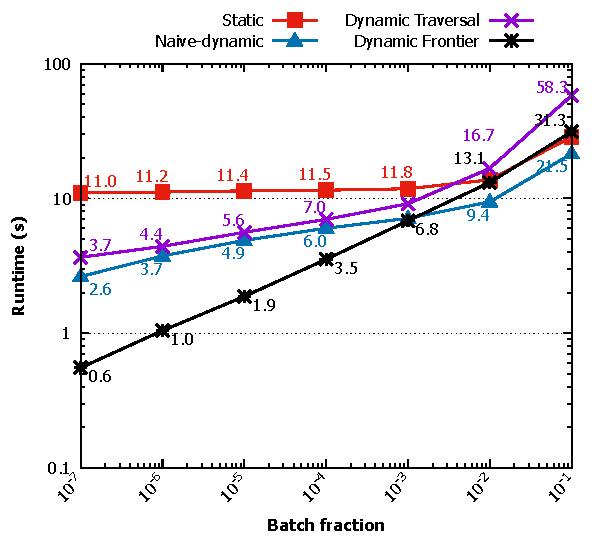
\includegraphics[width=0.38\linewidth]{out/insertions-runtime-mean.pdf}
  }
  \subfigure[Results on each graph]{
    \label{fig:insertions-runtime--all}
    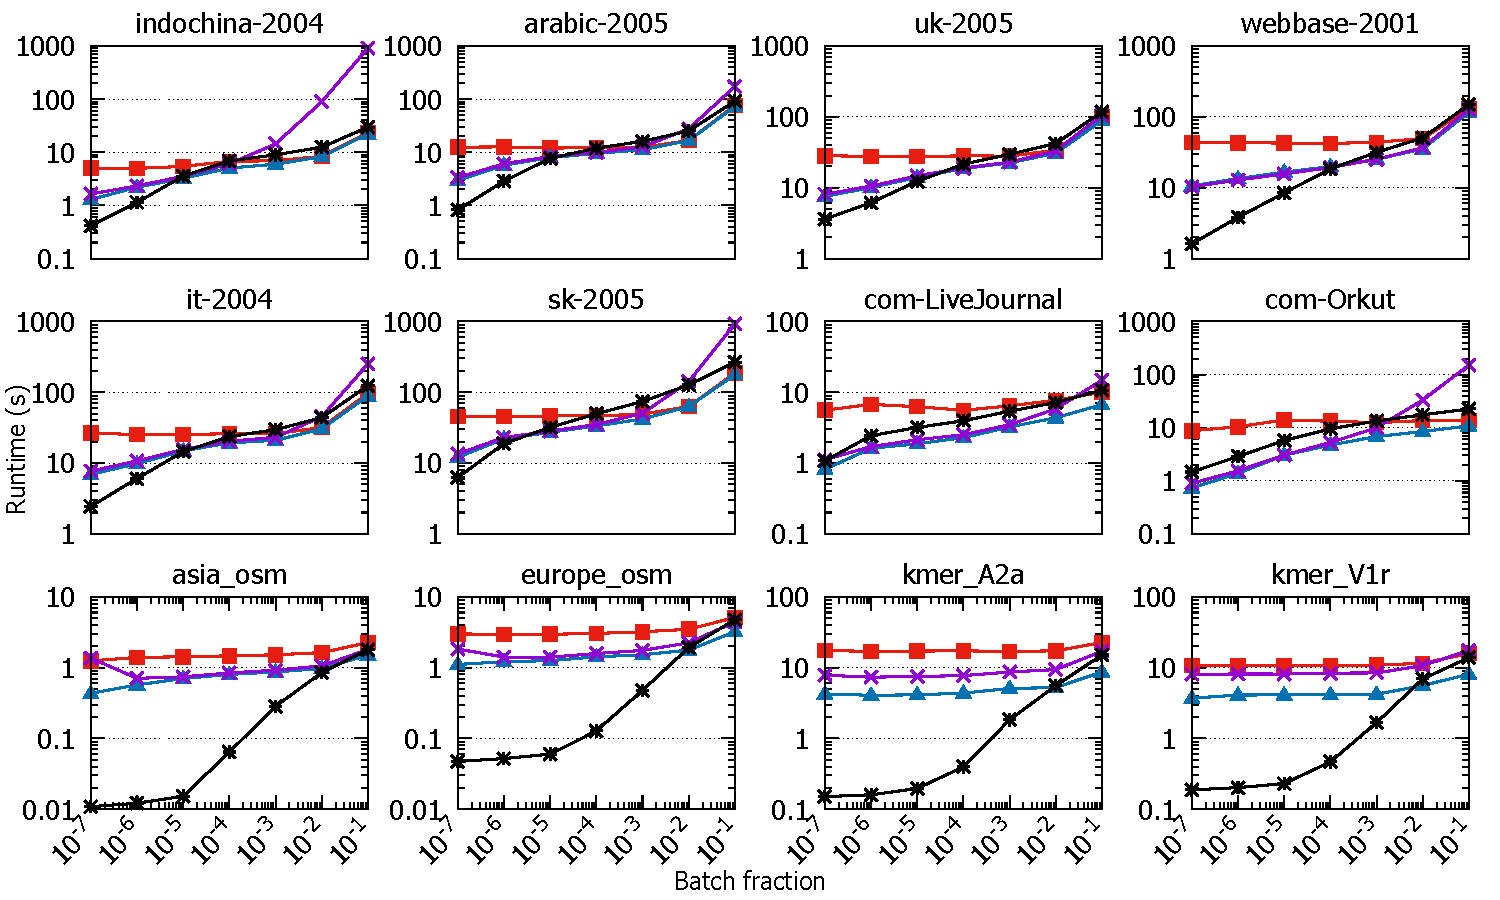
\includegraphics[width=0.58\linewidth]{out/insertions-runtime-all.pdf}
  } \\[-1ex]
  \caption{Runtime (logarithmic scale) for \textit{Static}, \textit{Naive-dynamic}, \textit{Dynamic Traversal}, and \textit{Dynamic Frontier} PageRank with batch updates exclusively comprising edge insertions, ranging from $10^{-7} |E|$ to $0.1 |E|$ in multiples of $10$ (logarithmic scale). The right figure details the runtime of each approach for individual graphs in the dataset, while the left figure displays overall runtimes --- using geometric mean for consistent scaling across graphs.}
  \label{fig:insertions-runtime}
\end{figure*}

\begin{figure*}[hbtp]
  \centering
  % \includegraphics[width=0.44\linewidth]{out/insertions-speedup-key.pdf}
  \subfigure[Overall result]{
    \label{fig:insertions-speedup--mean}
    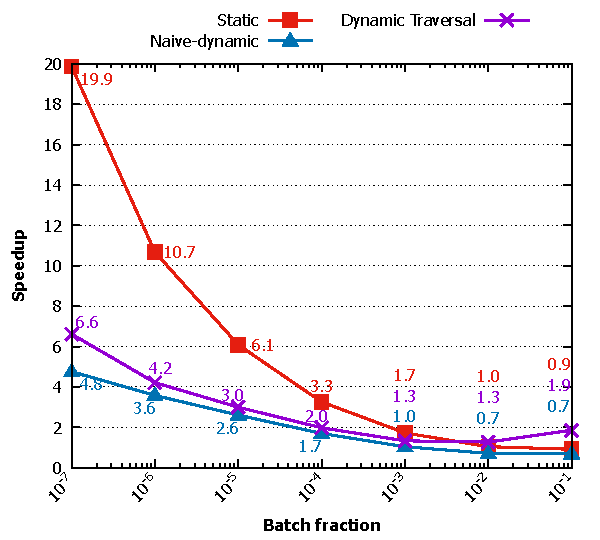
\includegraphics[width=0.38\linewidth]{out/insertions-speedup-mean.pdf}
  }
  \subfigure[Results on each graph]{
    \label{fig:insertions-speedup--all}
    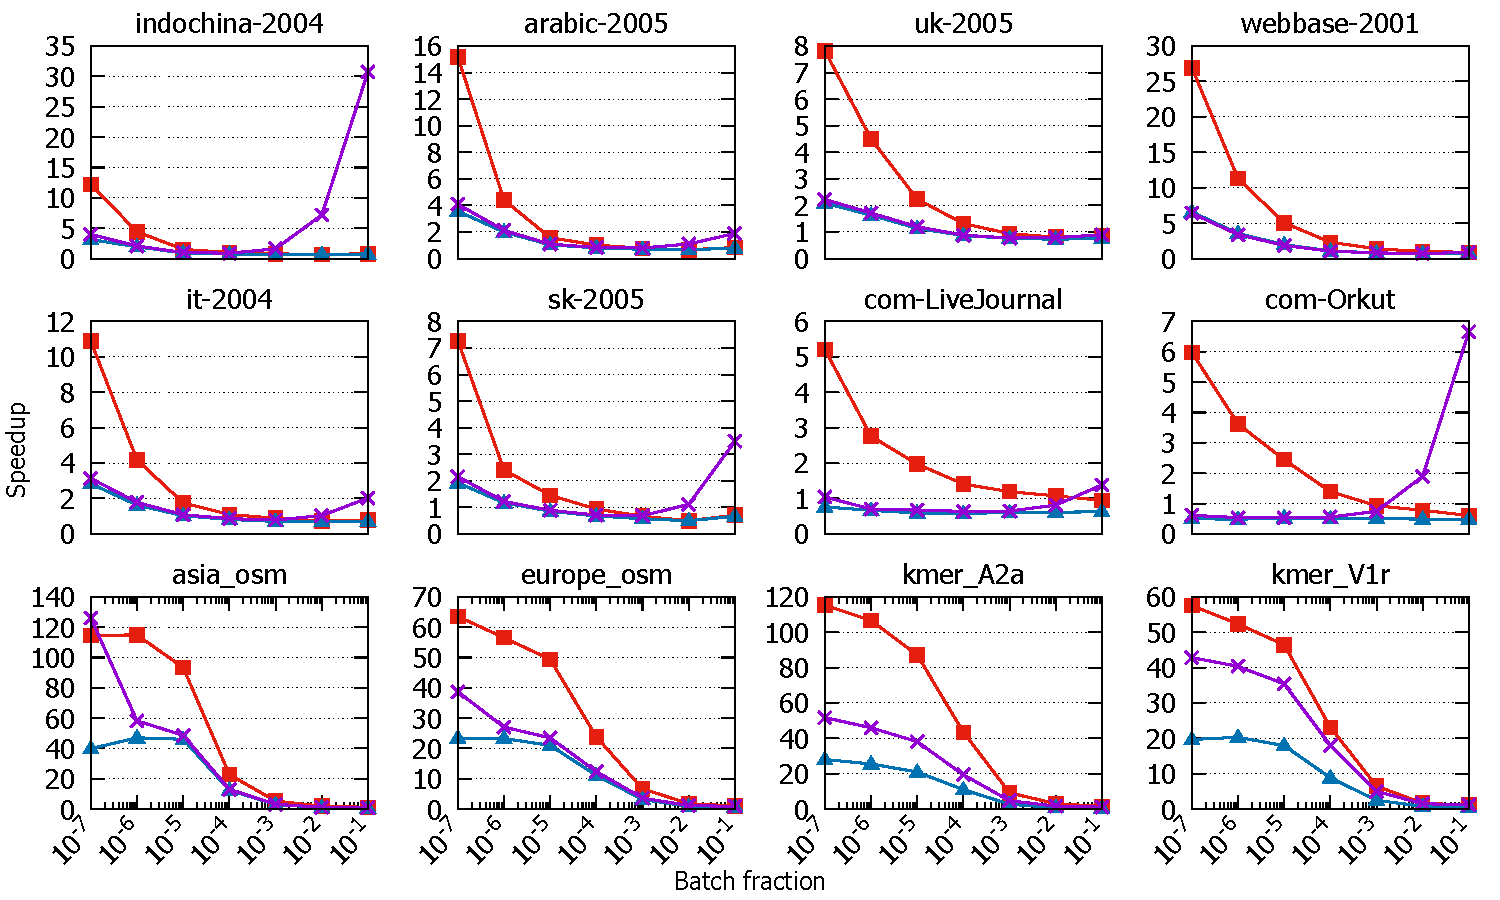
\includegraphics[width=0.58\linewidth]{out/insertions-speedup-all.pdf}
  } \\[-1ex]
  \caption{Speedup of \textit{Dynamic Frontier} PageRank with respect to \textit{Static}, \textit{Naive-dynamic}, and \textit{Dynamic Traversal} PageRank, on batch updates consisting solely of edge insertions ranging from $10^{-7} |E|$ to $0.1 |E|$ (logarithmic scale). The right figure depicts the speedup of \textit{Dynamic Frontier} PageRank in relation to each approach for individual graphs in the dataset, while the left figure highlights the overall speedup.}
  \label{fig:insertions-speedup}
\end{figure*}

\begin{figure*}[hbtp]
  \centering
  % \includegraphics[width=0.44\linewidth]{out/insertions-error-key.pdf}
  \subfigure[Overall result]{
    \label{fig:insertions-error--mean}
    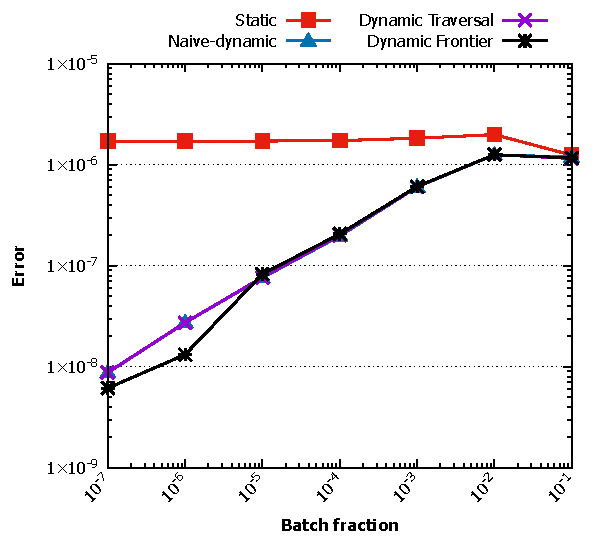
\includegraphics[width=0.38\linewidth]{out/insertions-error-mean.pdf}
  }
  \subfigure[Results on each graph]{
    \label{fig:insertions-error--all}
    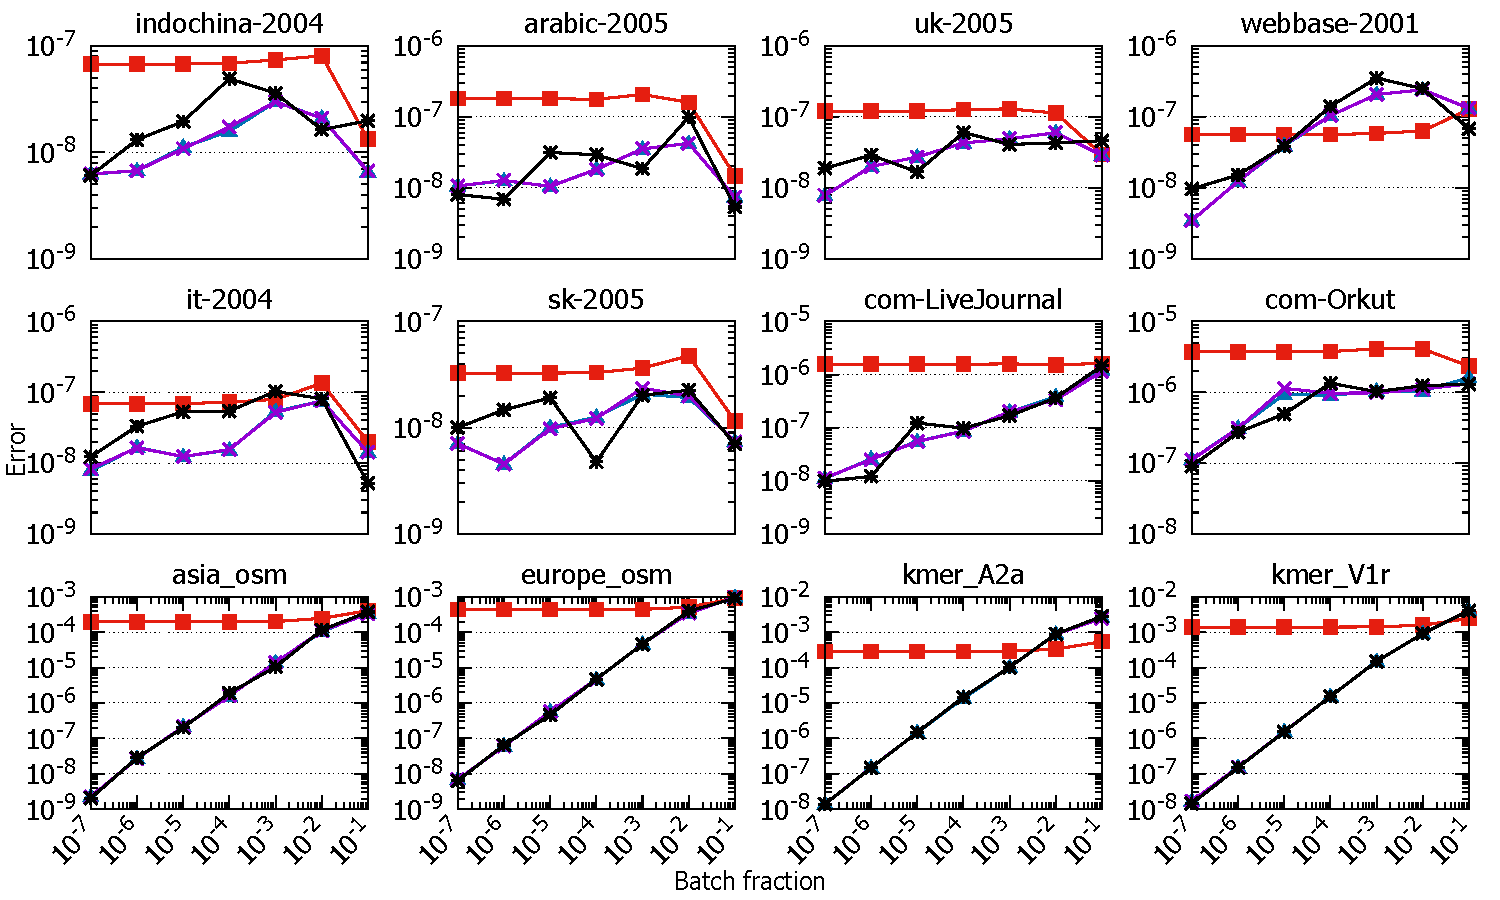
\includegraphics[width=0.58\linewidth]{out/insertions-error-all.pdf}
  } \\[-1ex]
  \caption{Error analysis comparing \textit{Static}, \textit{Naive-dynamic}, \textit{Dynamic Traversal}, and \textit{Dynamic Frontier} PageRank with a Reference Static PageRank (with a tolerance $\tau$ of $10^{-100}$ and limited to $500$ iterations) using $L1$-norm. Batch updates involve edge insertions ranging from $10^{-7} |E|$ to $0.1 |E|$ (logarithmic scale). The right figure illustrates the error specific to each approach for individual graphs in the dataset, while the left figure presents overall errors using the geometric mean for consistent scaling across graphs.}
  \label{fig:insertions-error}
\end{figure*}

\begin{figure*}[hbtp]
  \centering
  % \includegraphics[width=0.44\linewidth]{out/deletions-runtime-key.pdf}
  \subfigure[Overall result]{
    \label{fig:deletions-runtime--mean}
    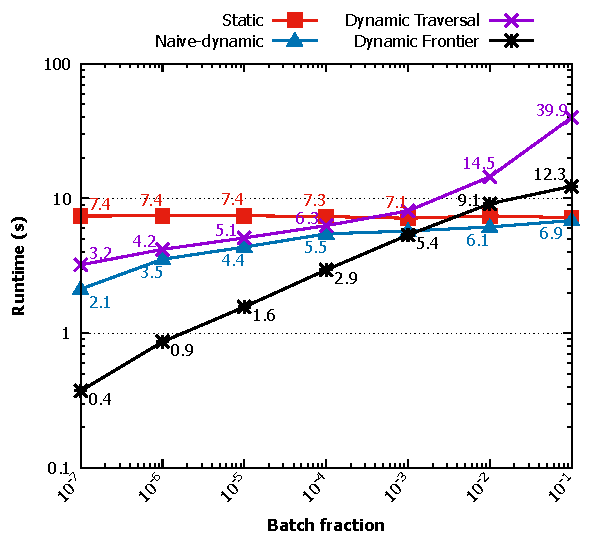
\includegraphics[width=0.38\linewidth]{out/deletions-runtime-mean.pdf}
  }
  \subfigure[Results on each graph]{
    \label{fig:deletions-runtime--all}
    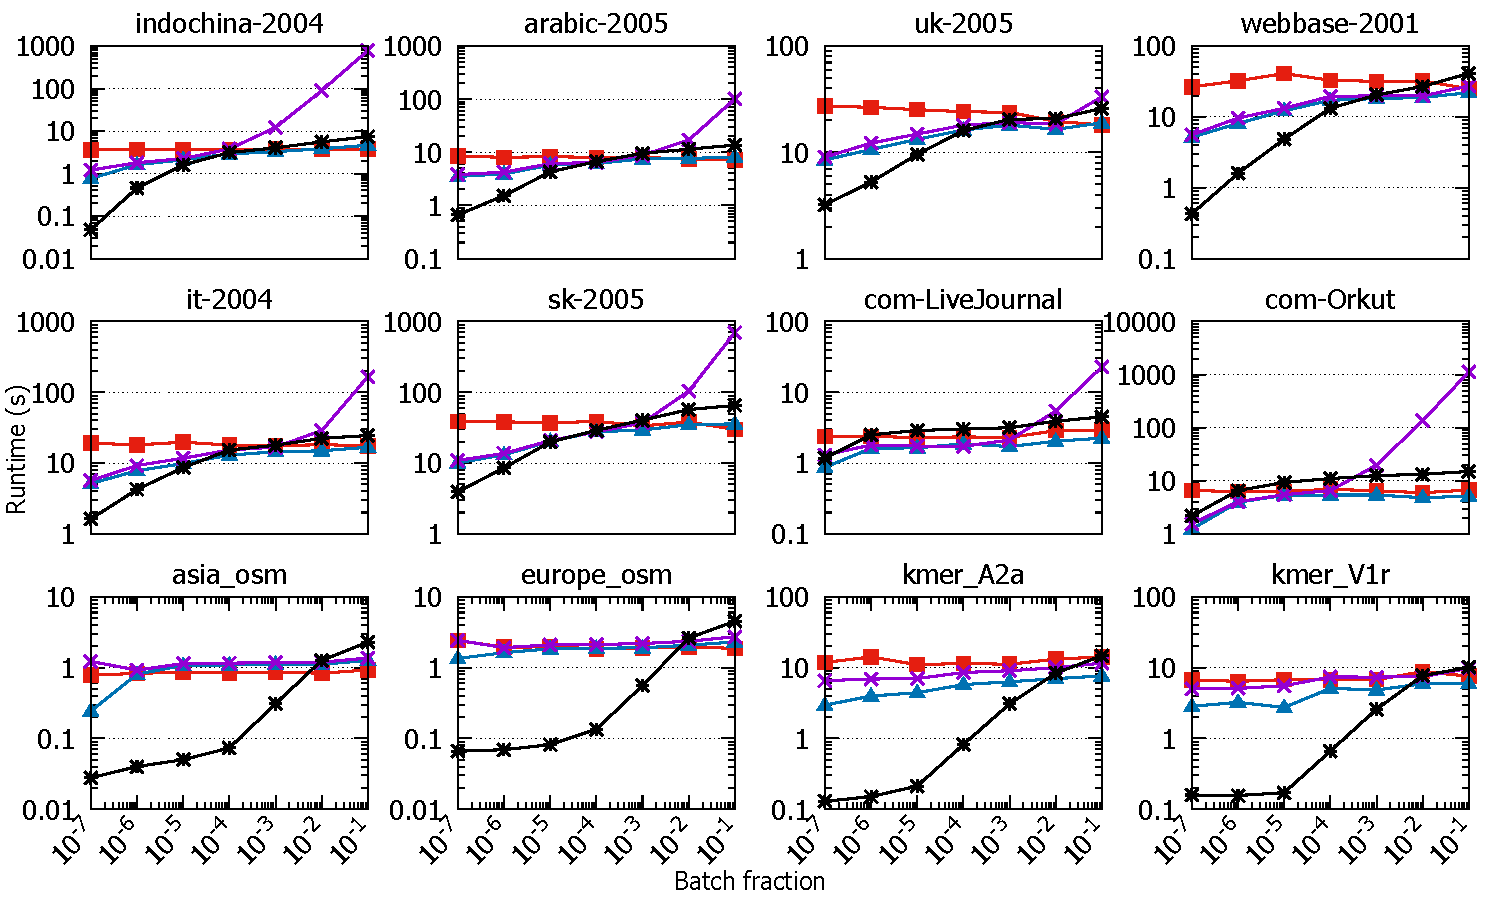
\includegraphics[width=0.58\linewidth]{out/deletions-runtime-all.pdf}
  } \\[-1ex]
  \caption{Deletions Time taken (solid lines), and modularity of communities obtained (dashed lines) along the Y2 axis, with X, X, and X (Algorithm X) on batch updates of increasing size from $10^{-7} |E|$ to $0.1 |E|$. Note that both axes are logarithmic. The numbers on the lines corresponding to X and X indicate the speedup of X over  the two algorithms, respectively.}
  \label{fig:deletions-runtime}
\end{figure*}

\begin{figure*}[hbtp]
  \centering
  % \includegraphics[width=0.44\linewidth]{out/deletions-speedup-key.pdf}
  \subfigure[Overall result]{
    \label{fig:deletions-speedup--mean}
    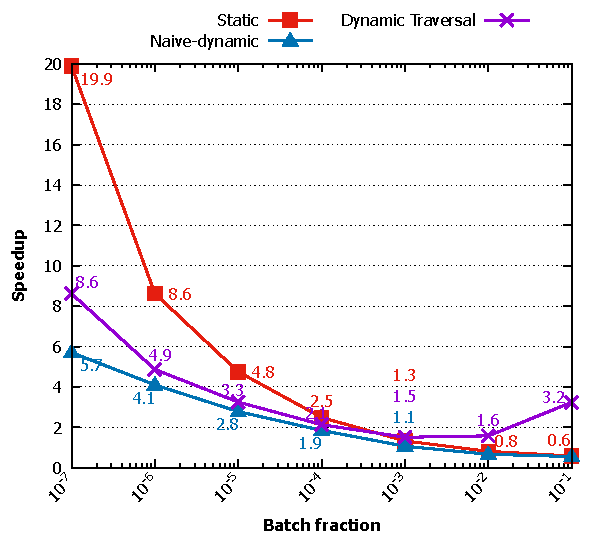
\includegraphics[width=0.38\linewidth]{out/deletions-speedup-mean.pdf}
  }
  \subfigure[Results on each graph]{
    \label{fig:deletions-speedup--all}
    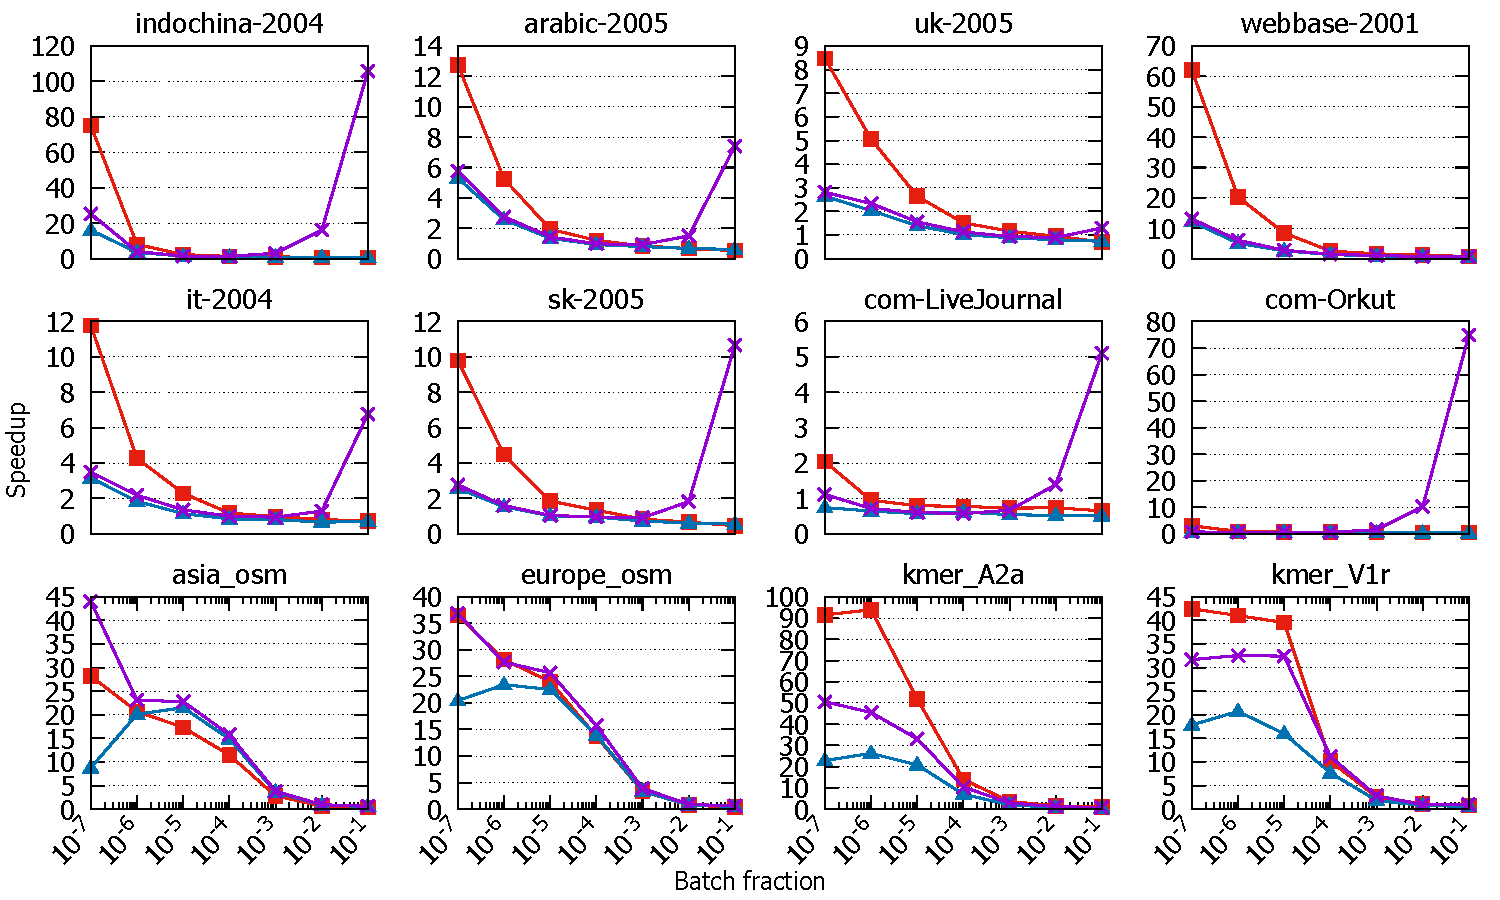
\includegraphics[width=0.58\linewidth]{out/deletions-speedup-all.pdf}
  } \\[-1ex]
  \caption{Speedup of \textit{Dynamic Frontier} PageRank in relation to \textit{Static}, \textit{Naive-dynamic}, and \textit{Dynamic Traversal} PageRank, on batch updates comprised solely of edge deletions ranging from $10^{-7} |E|$ to $0.1 |E|$ (logarithmic scale). The right figure illustrates the speedup of \textit{Dynamic Frontier} PageRank concerning each approach for individual graphs in the dataset, while the left figure emphasizes the overall speedup.}
  \label{fig:deletions-speedup}
\end{figure*}

\begin{figure*}[hbtp]
  \centering
  % \includegraphics[width=0.44\linewidth]{out/deletions-error-key.pdf}
  \subfigure[Overall result]{
    \label{fig:deletions-error--mean}
    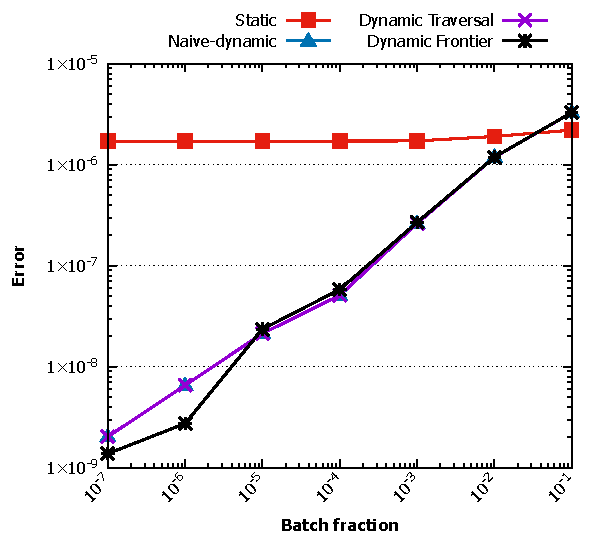
\includegraphics[width=0.38\linewidth]{out/deletions-error-mean.pdf}
  }
  \subfigure[Results on each graph]{
    \label{fig:deletions-error--all}
    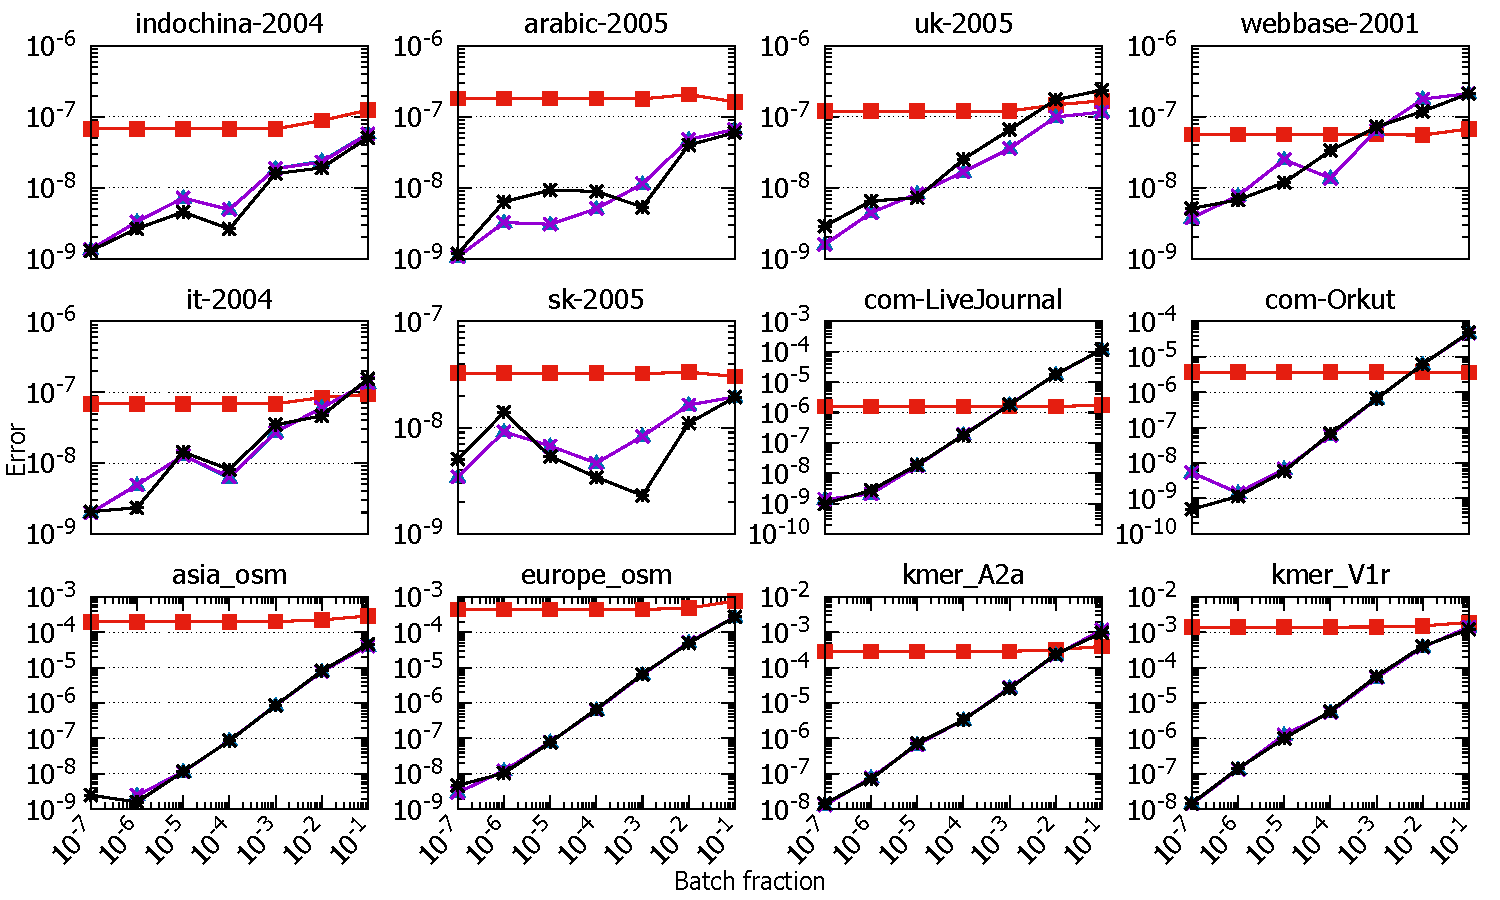
\includegraphics[width=0.58\linewidth]{out/deletions-error-all.pdf}
  } \\[-1ex]
  \caption{Deletions Time taken (solid lines), and modularity of communities obtained (dashed lines) along the Y2 axis, with X, X, and X (Algorithm X) on batch updates of increasing size from $10^{-7} |E|$ to $0.1 |E|$. Note that both axes are logarithmic. The numbers on the lines corresponding to X and X indicate the error of X over  the two algorithms, respectively.}
  \label{fig:deletions-error}
\end{figure*}

\begin{figure*}[hbtp]
  \centering
  % \includegraphics[width=0.44\linewidth]{out/8020-runtime-key.pdf}
  \subfigure[Overall result]{
    \label{fig:8020-runtime--mean}
    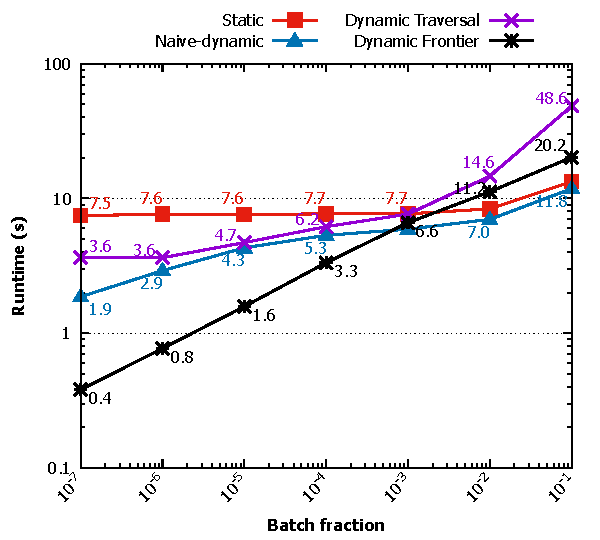
\includegraphics[width=0.38\linewidth]{out/8020-runtime-mean.pdf}
  }
  \subfigure[Results on each graph]{
    \label{fig:8020-runtime--all}
    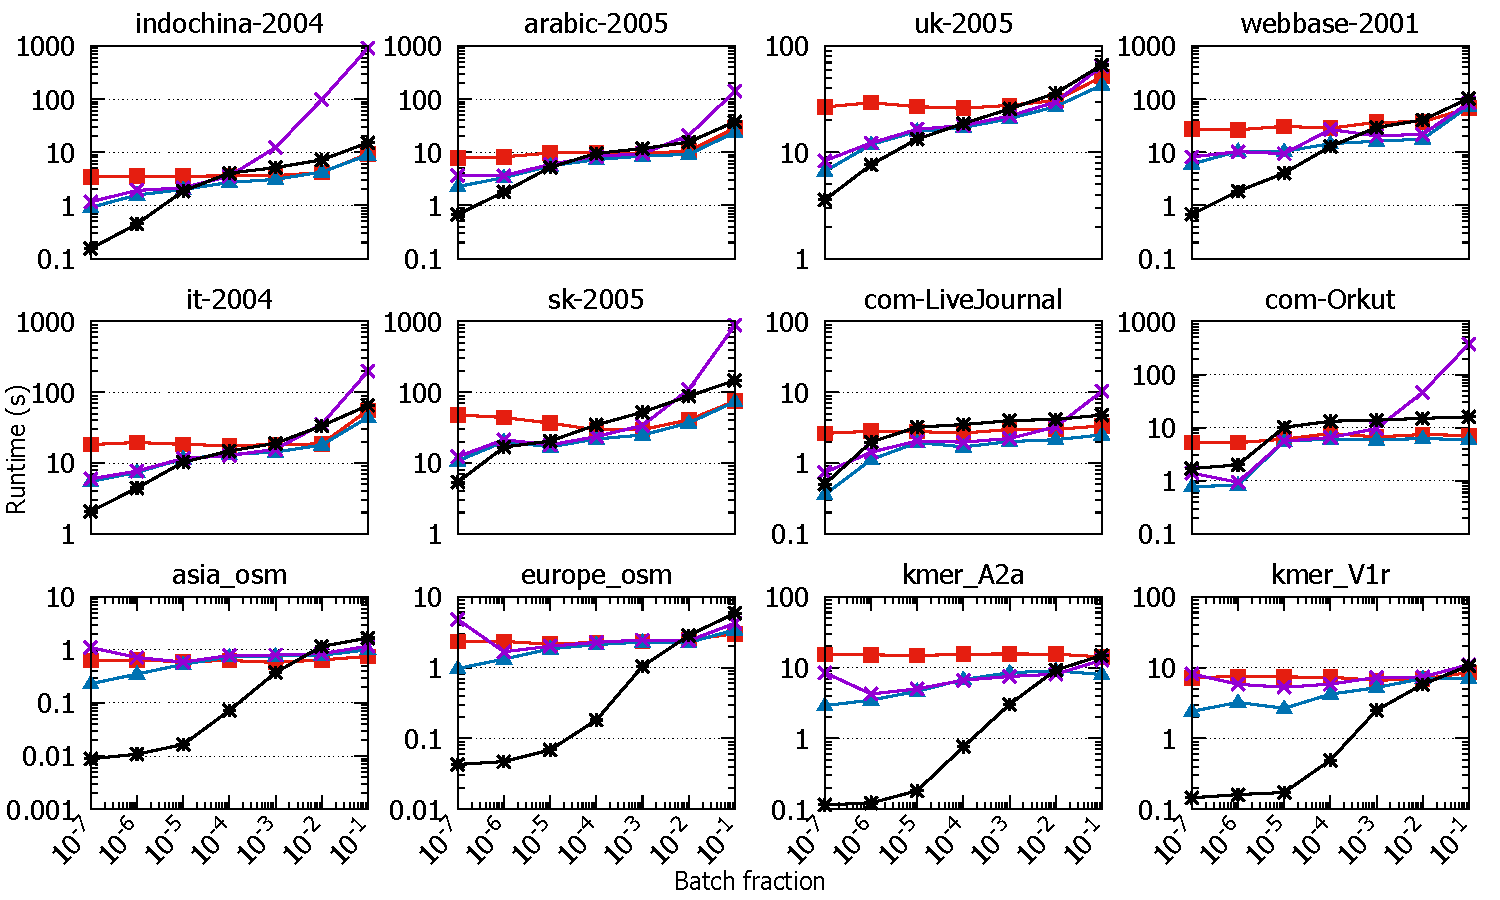
\includegraphics[width=0.58\linewidth]{out/8020-runtime-all.pdf}
  } \\[-1ex]
  \caption{8020 Time taken (solid lines), and modularity of communities obtained (dashed lines) along the Y2 axis, with X, X, and X (Algorithm X) on batch updates of increasing size from $10^{-7} |E|$ to $0.1 |E|$. Note that both axes are logarithmic. The numbers on the lines corresponding to X and X indicate the speedup of X over  the two algorithms, respectively.}
  \label{fig:8020-runtime}
\end{figure*}

\begin{figure*}[hbtp]
  \centering
  % \includegraphics[width=0.44\linewidth]{out/8020-speedup-key.pdf}
  \subfigure[Overall result]{
    \label{fig:8020-speedup--mean}
    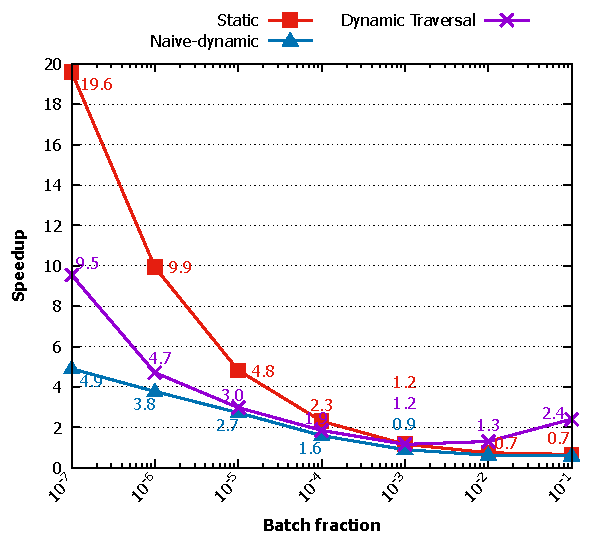
\includegraphics[width=0.38\linewidth]{out/8020-speedup-mean.pdf}
  }
  \subfigure[Results on each graph]{
    \label{fig:8020-speedup--all}
    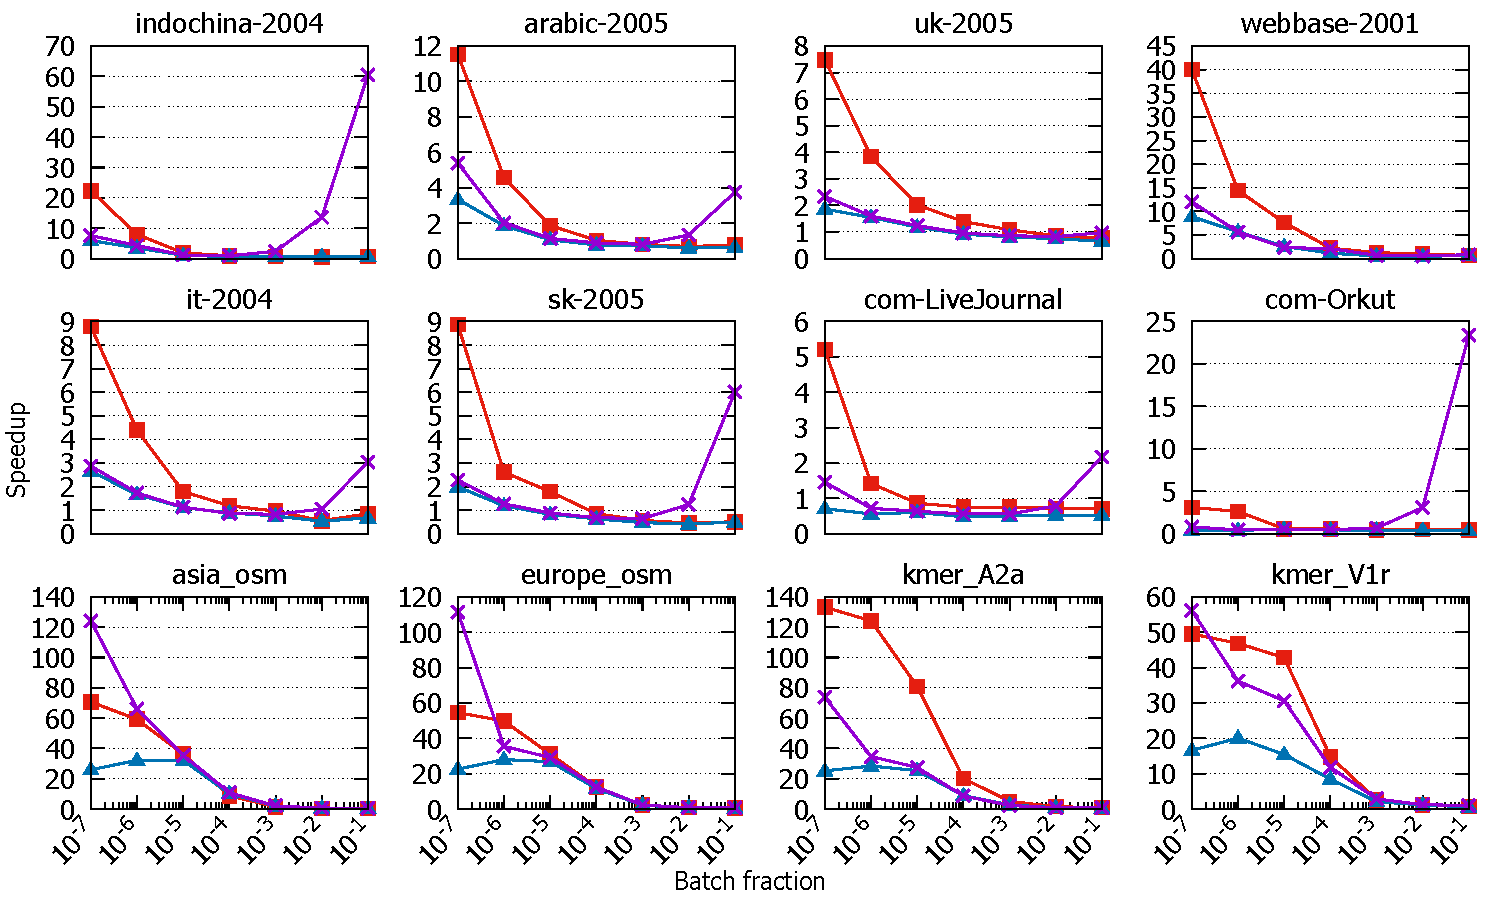
\includegraphics[width=0.58\linewidth]{out/8020-speedup-all.pdf}
  } \\[-1ex]
  \caption{8020 Time taken (solid lines), and modularity of communities obtained (dashed lines) along the Y2 axis, with X, X, and X (Algorithm X) on batch updates of increasing size from $10^{-7} |E|$ to $0.1 |E|$. Note that both axes are logarithmic. The numbers on the lines corresponding to X and X indicate the speedup of X over  the two algorithms, respectively.}
  \label{fig:8020-speedup}
\end{figure*}

\begin{figure*}[hbtp]
  \centering
  % \includegraphics[width=0.44\linewidth]{out/8020-error-key.pdf}
  \subfigure[Overall result]{
    \label{fig:8020-error--mean}
    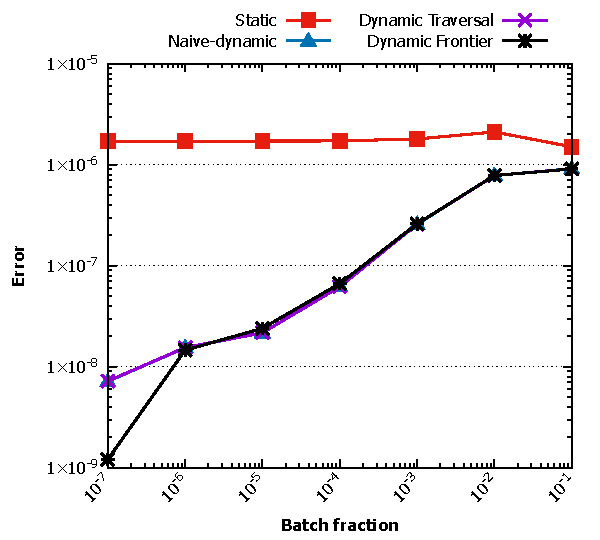
\includegraphics[width=0.38\linewidth]{out/8020-error-mean.pdf}
  }
  \subfigure[Results on each graph]{
    \label{fig:8020-error--all}
    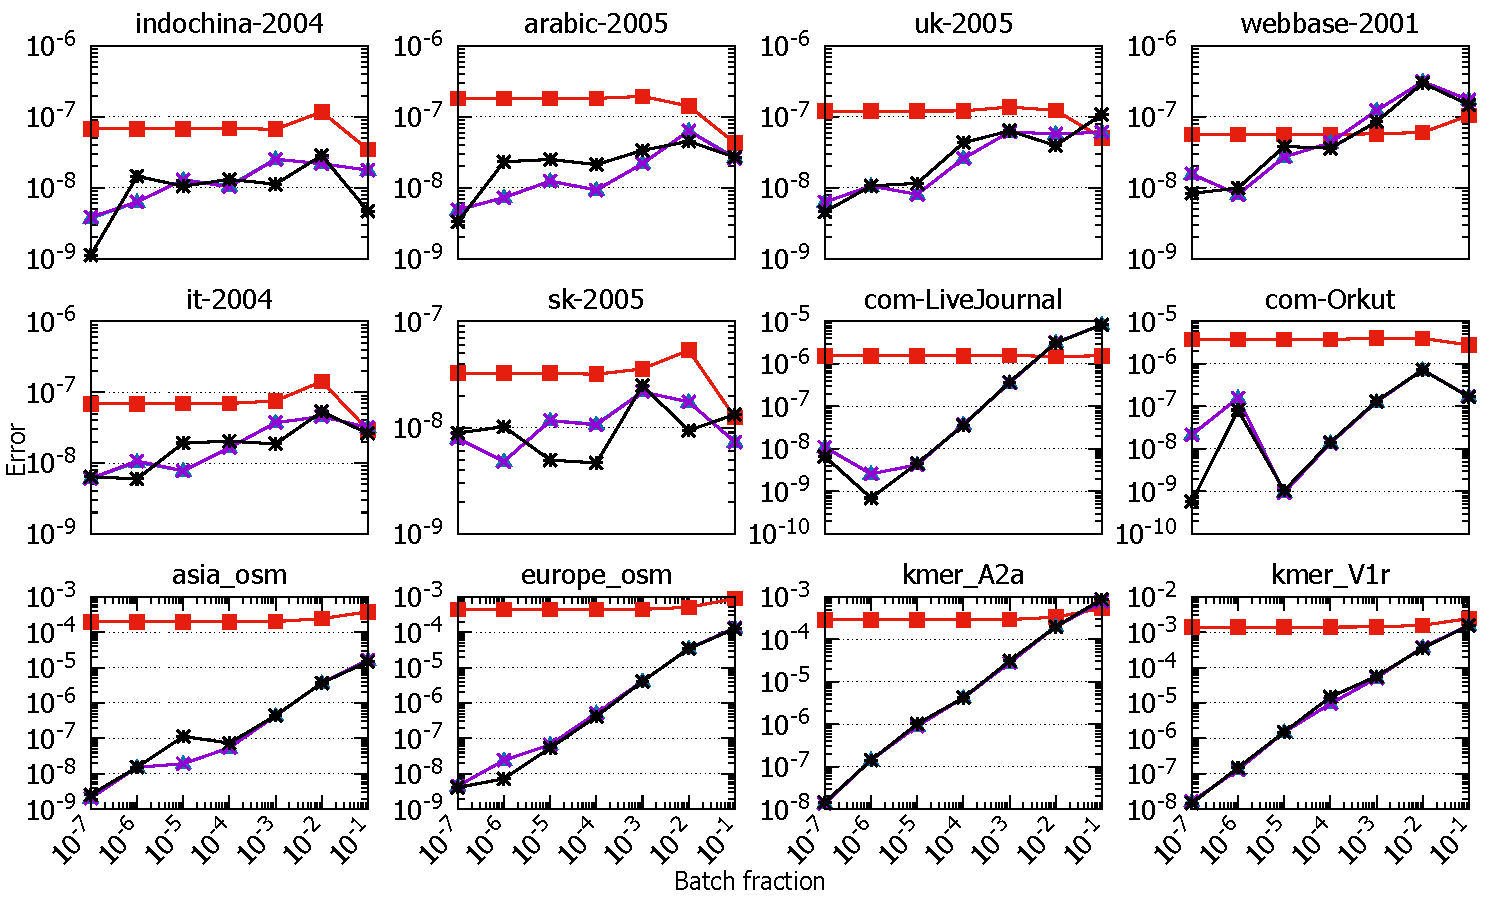
\includegraphics[width=0.58\linewidth]{out/8020-error-all.pdf}
  } \\[-1ex]
  \caption{Error comparison of \textit{Static}, \textit{Naive-dynamic}, \textit{Dynamic Traversal}, and \textit{Dynamic Frontier} PageRank with respect to a Reference Static PageRank (with a tolerance $\tau$ of $10^{-100}$ and limited to $500$ iterations), using $L1$-norm. Batch updates range from $10^{-7} |E|$ to $0.1 |E|$ (logarithmic scale), consisting of $80\%$ edge insertions and $20\%$ edge deletions to simulate realistic dynamic graph updates. The right figure depicts the error for each approach in relation to each graph, while the left figure showcases overall errors using geometric mean for consistent scaling across graphs.}
  \label{fig:8020-error}
\end{figure*}

\begin{figure}[!hbt]
  \centering
  \subfigure{
    \label{fig:measure-affected--batch}
    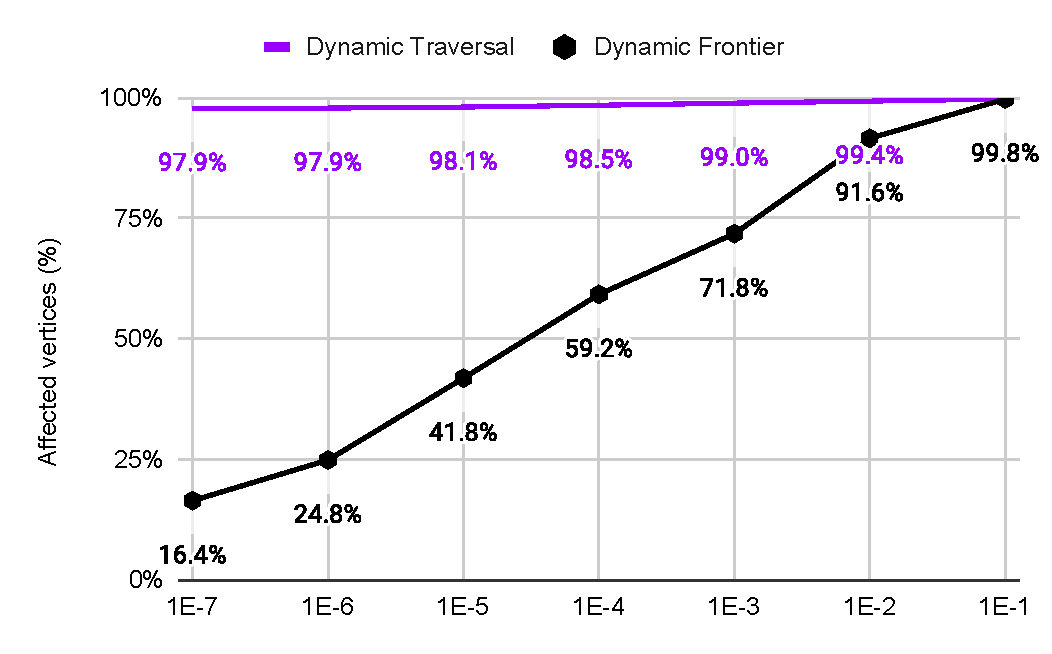
\includegraphics[width=0.98\linewidth]{out/measure-affected-batch.pdf}
  } \\[-2ex]
\caption{Average percentage of vertices marked as affected by \textit{Dynamic Traversal} and \textit{Dynamic Frontier} PageRank, with batch size increasing from $10^{-7} |E|$ to $0.1 |E|$ in multiples of $10$ (logarithmic scale), consisting purely of edge insertions. The \textit{Dynamic Frontier} approach marks affected vertices incrementally --- thus, the final percentage (at the end of all iterations) is depicted here.}
  \label{fig:measure-affected}
\end{figure}





\subsection{Performance of Dynamic Frontier PageRank}

We first study the performance of Dynamic Frontier PageRank on batch updates of size $10^{-7}|E|$ to $0.1|E|$ (in multiples of $10$), consisting purely of edge insertions, and compare it with Static, Naive-dynamic, and Dynamic Traversal PageRank. As mentioned above, the edge insertions are generated uniformly at random. Figure \ref{fig:insertions-runtime} plots the runtime of Static, Naive-dynamic, Dynamic Traversal, and Dynamic Frontier PageRank; Figure \ref{fig:insertions-speedup} plots the speedup of Dynamic Frontier PageRank with respect to Static, Naive-dynamic, and Dynamic Traversal PageRank; and Figure \ref{fig:insertions-error} plots the error in ranks obtained with Static, Naive-dynamic, Dynamic Traversal, and Dynamic Frontier PageRank with respect to ranks obtained from a reference Static PageRank (see Section \ref{sec:measurement}). In a similar manner, Figures \ref{fig:deletions-runtime}, \ref{fig:deletions-speedup}, and \ref{fig:deletions-error} present the runtime, speedup, and rank errors of each approach on batch updates consisting purely of edge deletions. Finally, Figures \ref{fig:8020-runtime}, \ref{fig:8020-speedup}, and \ref{fig:8020-error} present the runtime, speedup, and error with each approach on batch updates consisting of an $80\%$ / $20\%$ mix of edge insertions and deletions, in order to simulate realistic batch updates.


\subsubsection{Results with insertions-only batch updates}

Dynamic Frontier PageRank is on average $8.3\times$, $2.7\times$, and $3.4\times$ faster than Static, Naive-dynamic, and Dynamic Traversal PageRank on insertions-only batch updates of size $10^{-7}|E|$ to $10^{-3}|E|$, while obtaining ranks of better accuracy/error than Static PageRank, and of similar accuracy/error as Naive-dynamic and Dynamic Traversal PageRank. On road networks, and protein k-mer graphs, Dynamic Frontier PageRank is significantly faster than its competitors (Naive-dynamic and Dynamic Traversal PageRank).


\subsubsection{Results with deletions-only batch updates}

On deletions-only batch updates of size $10^{-7}|E|$ to $10^{-3}|E|$, Dynamic Frontier PageRank is on average $7.4\times$, $3.1\times$, and $4.1\times$ faster than Static, Naive-dynamic, and Dynamic Traversal PageRank, while obtaining ranks of better accuracy/error than Static PageRank (for batch sizes less than $0.1|E|$), and of similar accuracy/error as Naive-dynamic and Dynamic Traversal PageRank. On \textit{indochina-2004}, \textit{webbase-2001}, road networks, and protein k-mer graphs, Dynamic Frontier PageRank is significantly faster than its competitors (Naive-dynamic and Dynamic Traversal PageRank).


\subsubsection{Results with 80\%-20\% mix batch updates}

On batch updates of size $10^{-7}|E|$ to $10^{-3}|E|$, consisting of $80\%$ insertions and $20\%$ deletions, Dynamic Frontier PageRank is on average $7.6\times$, $2.8\times$, and $4.1\times$ faster than Static, Naive-dynamic, and Dynamic Traversal PageRank, while obtaining ranks of better accuracy/error than Static PageRank, and of similar accuracy/error as Naive-dynamic and Dynamic Traversal PageRank. Similar to deletions-only batch updates, Dynamic Frontier PageRank outperforms its competitors (Naive-dynamic and Dynamic Traversal PageRank) on \textit{indochina-2004}, \textit{webbase-2001}, road networks, and protein k-mer graphs.
% This seems to be associated to sparsity of the graphs as Dynamic Frontier PageRank performing well on sparse graphs.


\subsubsection{Results with temporal graphs}

We also attempt Static, Naive-dynamic, Dynamic Traversal, and Dynamic Frontier PageRank on temporal graphs found in the Stanford Large Network Dataset Collection \cite{snap14}. On some temporal graphs, Dynamic Frontier PageRank does not outperform its competitors with a frontier tolerance of $\tau_f = \tau / 10^5$, where $\tau$ is the iteration tolerance. However, choosing a lower $\tau_f$ of $\tau / 10$ or $\tau / 100$ allows it achieve good performance. Thus, the choice of frontier tolerance $\tau_f$, possibly in addition to how the frontier of affected vertices is expanded, is dependent upon the nature of the batch update. We plan to explore this in the future.


\subsubsection{Comparison of vertices marked as affected}

Figure \ref{fig:measure-affected} shows the total number of vertices marked as affected (average) by Dynamic Traversal and Dynamic Frontier PageRank on batch updates of size $10^{-7}|E|$ to $0.1|E|$, consisting exclusively of edge insertions. The Dynamic Frontier approach marks affected vertices incrementally --- thus, the final percentage (at the end of all iterations) is depicted in the figure. It is observed that Dynamic Traversal PageRank marks a higher percentage of vertices as affected, even for small batch updates.\ignore{This is likely due the randomly generated edges in the batch update being part of large Strongly Connected Components (SCCs), or due to a large number of such SCCs being reachable from the vertices that are part of the batch update.} In contrast, Dynamic Frontier PageRank marks far fewer vertices as affected, as it incrementally expands the affected region of the graph only after the rank of an affected vertex changes by a substantial amount, i.e., by frontier tolerance $\tau_f = \tau / 10^5$, where $\tau$ is the iteration tolerance (using $L\infty$-norm). In addition, as Dynamic Frontier PageRank incrementally marks vertices as affected, the actual work performed by the algorithm is lower than that indicated by the percentage of affected vertices in Figure \ref{fig:measure-affected}.

\begin{figure}[!hbt]
  \centering
  \subfigure{
    \label{fig:strong-scaling--speedup}
    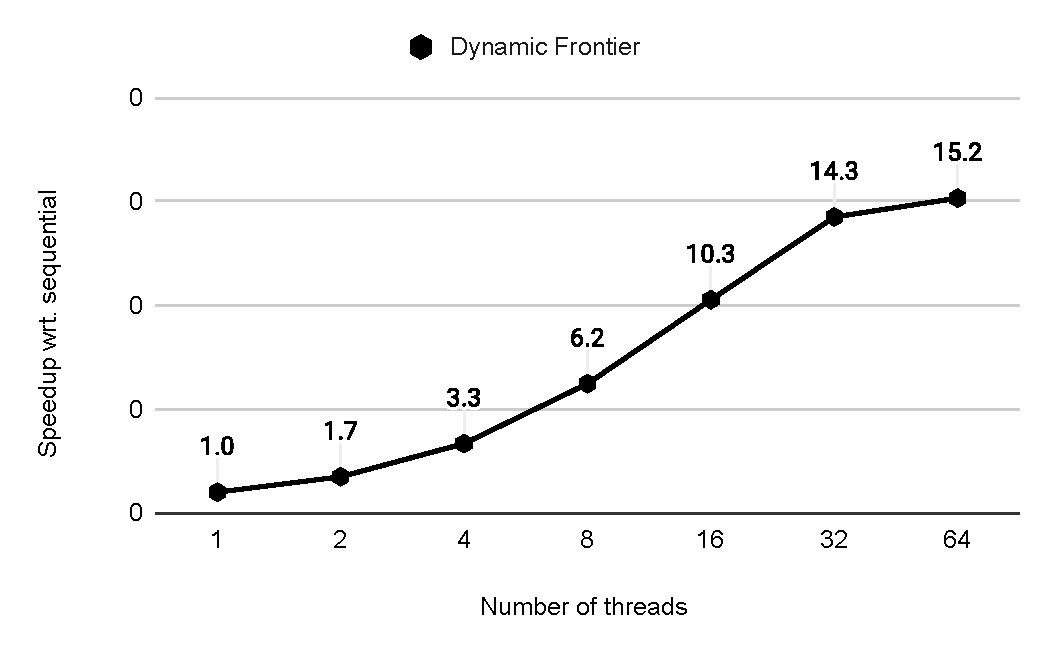
\includegraphics[width=0.98\linewidth]{out/strong-scaling-speedup.pdf}
  } \\[-2ex]
  \caption{Average speedup of \textit{Dynamic Frontier} PageRank with increasing number of threads (in multiples of $2$), on a batch size of $10^{-4}|E|$ (consisting purely of edge insertions).}
  \label{fig:strong-scaling}
\end{figure}





\subsection{Strong Scaling of Dynamic Frontier PageRank}

Finally, we study the strong-scaling behavior of Dynamic Frontier PageRank on batch updates of a fixed size of $10^{-4} |E|$, consisting purely of edge insertions. Here, we measure the speedup of Dynamic Frontier PageRank with an increasing number of threads from $1$ to $64$ in multiples of $2$ with respect to a single-threaded execution of the algorithm. This is repeated for each graph in the dataset, and the results are averaged (using geometric mean).

The results are shown in Figure \ref{fig:strong-scaling}. With $16$ threads, Dynamic Frontier PageRank achieves an average speedup of $10.3\times$, compared to a single-threaded execution, indicating a performance increase of $1.8\times$ for every doubling of threads. At $32$ and $64$ threads, Dynamic Frontier PageRank is affected by NUMA effects (the $64$-core processor we use has $4$ NUMA domains), resulting in a speedup of only $14.3\times$ and $15.2\times$ respectively.

\ignore{\begin{figure}[!hbt]
  \centering
  \subfigure{
    \label{fig:weak-scaling--speedup}
    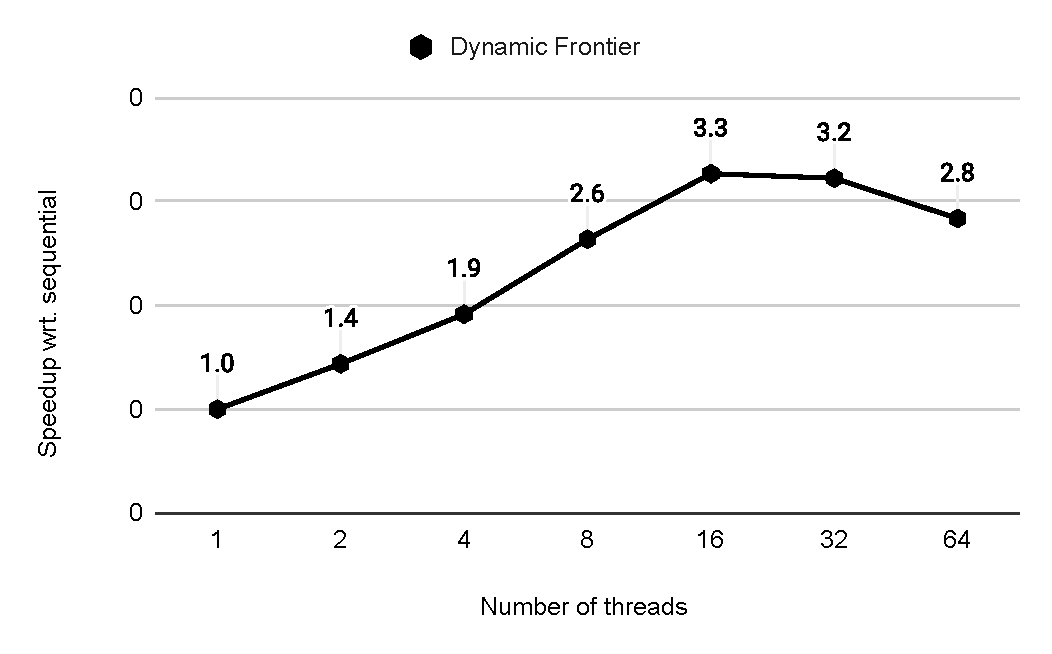
\includegraphics[width=0.98\linewidth]{out/weak-scaling-speedup.pdf}
  } \\[-2ex]
  \caption{Average speedup of \textit{Dynamic Frontier} PageRank with increasing number of threads (in multiples of $2$), on a batch sizes of $10^{-4}|E|$ to $6.4\times10^{-3}|E|$ (consisting purely of edge insertions), increasing in multiples of $2$ in tandem with the increase in the number of threads.}
  \label{fig:weak-scaling}
\end{figure}
}


\section{Conclusion}
\label{sec:conclusion}
The popularity of PageRank as a centrality metric stems from its ability to assign importance to graph nodes based on their neighbors and scores. In recent years, there has been increasing research focus on computing PageRank for dynamic graphs, where the graphs evolve due to edge insertions and deletions. Simultaneously, the trend of increasing core count in multicore architectures has raised concerns regarding random thread delays and failures. To tackle these challenges, fault-tolerant algorithms that can efficiently function even in the presence of thread delays or crashes are essential.

In this paper we presented the design of a lock-free fault-tolerant PageRank algorithm in the batch dynamic setting, where edge deletions and insertions are applied to the given dynamic graph in batches. First, we introduced our \textit{Static Barrier-free} PageRank (\StaBarf{}) which tolerates random thread delays or crashes. It is simpler in design compared to Eedi et al.'s \textit{Wait-free} version of \textit{Barrier-free} PageRank \cite{rank-eedi22}, and exhibits a $14\%$ improvement in speed to Eedi et al.'s \textit{No-Sync} version of \textit{Barrier-free} PageRank (which is not tolerant to thread crashes). We then adapted our improved \textit{Barrier-free} PageRank to two well-known dynamic PageRank algorithms, namely, \textit{Naive-dynamic} and \textit{Dynamic Traversal}. However, our results indicated that \textit{Dynamic Traversal} approach does not have good performance.

Next, we discussed our \textit{Dynamic Frontier} approach, which incrementally identifies affected vertices that are likely to change their ranks with minimal overhead, in the batch dynamic setting. We integrated it with our fault-tolerant \textit{Barrier-free} PageRank (\FroBarf{}). \FroBarf{} is fast and lock-free. Experimental results indicate that \FroBarf{} is, on average, $4.6\times$ faster than \textit{Naive-dynamic Barrier-free} PageRank (\NaiBarf{}). Simulation studies further show that \FroBarf{} maintains good performance in the presence of random thread delays and can tolerate random thread crashes. In future, we plan to study how to tolerate arbitrary hardware faults in other hardware as well, such as GPUs and ML accelerators.
% We anticipate this to be useful in systems which operate in harsh environments. In the future, we would like to explore the applicability of the proposed technique to other graph algorithms such as betweenness centrality.


%% The acknowledgments section.
\begin{acks}
I would like to thank Prof. Kishore Kothapalli, Prof. Dip Sankar Banerjee, Vincent Traag, Geerten Verweij, and Fabian Nguyen for their support.
\end{acks}

%% Bibliography style to be used, and the bibliography file.
\bibliographystyle{ACM-Reference-Format}
\bibliography{main}

\end{document}
\endinput
%% End of file.




%% NOTES:
%% - Parallelization seems to be not efficient for small batch updates.
%% - Discuss about conflicting updates
%% - 


%% TODO:
%% - Scale up the size of the graphs
%% - Move experiments to a better server
%% - Include a weak- and strong- scalabiilty plot: run the expt from 2 to 128 threads
%% - overall space planning
%% - add a few lines on novelty of the paper.
%% - table comparison of related work
%% - Include a section on preliminaries that talks about the various algorithmic ideas (Louvain, Label Propagation)

%% Workplan:
%% - KK -- Read Introduction, Related Work,
%% - Dip Sankar -- Approach -- summarize the main algorithmic ideas,
%% - Subhajit -- Results -- Plots, scalability, Dataset, experiments, implementation details,
